\documentclass[table]{beamer}
%[]中可以使用draft、handout、screen、transparency、trancompress、compress等参数

%指定beamer的模式与主题
\mode<presentation>
{
  \usetheme{Madrid}
%\usetheme{Boadilla}
%\usecolortheme{default}
%\usecolortheme{orchid}
%\usecolortheme{whale}
%\usefonttheme{professionalfonts}
}

%\usetheme{Madrid}
%这里还可以选择别的主题:Bergen, Boadilla, Madrid, AnnArbor, CambridgeUS, Pittsburgh, Rochester, Warsaw, ...
%有导航栏的Antibes, JuanLesPins, Montpellier, ...
%有内容的Berkeley, PaloAlto, Goettingen, Marburg, Hannover, ...
%有最小导航栏的Berlin, Ilmenau, Dresden, Darmstadt, Frankfurt, Singapore, Szeged, ...
%有章和节表单的Copenhagen, Luebeck, Malmoe, Warsaw, ...

%\usecolortheme{default}
%设置内部颜色主题(这些主题一般改变block里的颜色);这个主题一般选择动物来命名
%这里还可以选择别的颜色主题,如默认的和有特别目的的颜色主题default,structure,sidebartab,全颜色主题albatross,beetle,crane,dove,fly,seagull,wolverine,beaver

%\usecolortheme{orchid}
%设置外部颜色主题(这些主题一般改变title里的颜色);这个主题一般选择植物来命名
%这里还可以选择别的颜色主题,如默认的和有特别目的的颜色主题lily,orchid,rose

%\usecolortheme{whale}
%设置字体主题;这个主题一般选择海洋动物来命名
%这里还可以选择别的颜色主题,如默认的和有特别目的的颜色主题whale,seahorse,dolphin

%\usefonttheme{professionalfonts}
%类似的还可以定义structurebold,structuresmallcapsserif,professionalfonts


% 控制 beamer 的风格,可以根据自己的爱好修改
%\usepackage{beamerthemesplit} %使用 split 风格
%\usepackage{beamerthemeshadow} %使用 shadow 风格
%\usepackage[width=2cm,dark,tab]{beamerthemesidebar}

%插入音标
\usepackage{tipa}
\AtBeginDocument{
  \renewcommand\textipa{\fontencoding{T3}\selectfont}
}
\AtBeginDocument{
  \renewcommand\textipa[2][r]{{\fontfamily{cm#1}\tipaencoding #2}}
}
\renewenvironment{IPA}[1][r]
 {\fontfamily{cm#1}\tipaencoding}
 {}

% 设定英文字体
%\usepackage{fontspec}
\usepackage[no-math]{fontspec}
\setmainfont{Times New Roman}
\setsansfont{Arial}
\setmonofont{Courier New}

% 设定中文字体
\usepackage[BoldFont,SlantFont,CJKchecksingle,CJKnumber]{xeCJK}
%\setCJKmainfont[BoldFont={Adobe Heiti Std},ItalicFont={Adobe Kaiti Std}]{Adobe Song Std}
\setCJKmainfont[BoldFont={Adobe Heiti Std},ItalicFont={Adobe Kaiti Std}]{WenQuanYi Micro Hei}
\setCJKsansfont{Adobe Heiti Std}
\setCJKmonofont{Adobe Fangsong Std}
\punctstyle{hangmobanjiao}

\defaultfontfeatures{Mapping=tex-text}
\usepackage{xunicode}
\usepackage{xltxtra}

\XeTeXlinebreaklocale "zh"
\XeTeXlinebreakskip = 0pt plus 1pt minus 0.1pt

\usepackage{setspace}
\usepackage{colortbl,xcolor}
\usepackage{hyperref}
%\hypersetup{xetex,bookmarksnumbered=true,bookmarksopen=true,pdfborder=1,breaklinks,colorlinks,linkcolor=blue,filecolor=black,urlcolor=cyan,citecolor=green}
\hypersetup{xetex,bookmarksnumbered=true,bookmarksopen=true,pdfborder=1,breaklinks,colorlinks,linkcolor=cyan,filecolor=black,urlcolor=blue,citecolor=green}

% 插入图片
\usepackage{graphicx}
\graphicspath{{figures/}}
% 图文混排
\usepackage{picins}
\usepackage{floatflt}

% 可能用到的包
\usepackage{amsmath,amssymb}
%插入多媒体
%\usepackage{media9}
%\usepackage{movie15}
\usepackage{multimedia}
\usepackage{multicol}
\usepackage{multirow}

% 定义一些自选的模板,包括背景、图标、导航条和页脚等,修改要慎重
% 设置背景渐变由10%的红变成10%的结构颜色
%\beamertemplateshadingbackground{red!10}{structure!10}
%\beamertemplatesolidbackgroundcolor{white!90!blue}
% 使所有隐藏的文本完全透明、动态,而且动态的范围很小
\beamertemplatetransparentcovereddynamic
% 使itemize环境中变成小球,这是一种视觉效果
\beamertemplateballitem
% 为所有已编号的部分设置一个章节目录,并且编号显示成小球
\beamertemplatenumberedballsectiontoc
% 将每一页的要素的要素名设成加粗字体
\beamertemplateboldpartpage

% item逐步显示时,使已经出现的item、正在显示的item、将要出现的item呈现不同颜色
\def\hilite<#1>{
 \temporal<#1>{\color{gray}}{\color{blue}}
    {\color{blue!25}}
}

\renewcommand{\today}{\number\year 年 \number\month 月 \number\day 日}

%五角星
\usepackage{MnSymbol}

%去除图表标题中的figure等
\usepackage{caption}
\captionsetup{labelformat=empty,labelsep=none}

\usepackage{tabu}
\usepackage{multirow}
%表格自动换行
\usepackage{tabularx} 

% 千分号
%\usepackage{textcomp}

%罗马数字
\makeatletter
\newcommand{\rmnum}[1]{\romannumeral #1}
\newcommand{\Rmnum}[1]{\expandafter\@slowromancap\romannumeral #1@}
\makeatother

%分栏
\usepackage{multicol}

%\usepackage{enumitem}
%\usepackage{enumerate}

%键盘
\usepackage{keystroke}

%插入源代码
\usepackage{listings}
\lstset{
  language=bash,                  % 程序语言名称:TeX, Perl, R, sh, bash, Awk
  basicstyle=\normalsize\tt,      %\tt指monospace字体族,程序源代码使用此族字体表示更加美观
  numbers=left,                   % 行号位置(左侧)
  numberstyle=\small,             % 行号字体的字号
  stepnumber=1,                   % 行号的显示步长
  numbersep=5pt,                  % 行号与代码间距
  backgroundcolor=\color{white},  % 背景色;需要 \usepackage{color}
  showspaces=false,               % 不显示空格
  showstringspaces=false,         % 不显示代码字符串中的空格标记
  showtabs=false,                 % 不显示 TAB
  tabsize=4, 
  frame=shadowbox,                % 把代码用带有阴影的框圈起来
  captionpos=b,                   % 标题位置
  breaklines=true,                % 对过长的代码自动断行
  breakatwhitespace=false,        % 断行只在空格处
  extendedchars=false,            % 解决代码跨页时,章节标题,页眉等汉字不显示的问题
  %escapeinside={\%*}{*},         % 跳脱字符,添加注释,暂时离开 listings 
  %escapeinside=``,
  commentstyle=\color{red!50!green!50!blue!50}\tt,  %浅灰色的注释
  rulesepcolor=\color{red!20!green!20!blue!20},     %代码块边框为淡青色
  keywordstyle=\color{blue!70}\bfseries\tt,         %代码关键字的颜色为蓝色,粗体
  identifierstyle=\tt,
  stringstyle=\tt,                % 代码字符串的特殊格式
  keepspaces=true,
  breakindent=1em,
  %breakindent=22pt,
  %breakindent=4em,
  breakautoindent=true,
  flexiblecolumns=true,
  aboveskip=1em,                  %代码块边框
  xleftmargin=2em,
  xrightmargin=2em
}

%\setbeamercolor{alerted text}{fg=magenta}
\setbeamercolor{bgcolor}{fg=yellow,bg=cyan}
%\setbeamercolor{itemize/enumerate body}{fg=green}

\begin{document}

%\includeonlyframes{current}

\logo{
\includegraphics[height=0.08\textwidth]{tijmu.png}}

% 在每个Section前都会加入的Frame
\AtBeginSection[]
{
  \begin{frame}<beamer>
    %\frametitle{Outline}
    \frametitle{教学提纲}
    \setcounter{tocdepth}{3}
    \begin{multicols}{2}
      \tableofcontents[currentsection,currentsubsection]
      %\tableofcontents[currentsection]
    \end{multicols}
  \end{frame}
}
% 在每个Subsection前都会加入的Frame
\AtBeginSubsection[]
{
  \begin{frame}<beamer>
%%\begin{frame}<handout:0>
%% handout:0 表示只在手稿中出现
    \frametitle{教学提纲}
    \setcounter{tocdepth}{3}
    \begin{multicols}{2}
    \tableofcontents[currentsection,currentsubsection]
    \end{multicols}
%% 显示在目录中加亮的当前章节
  \end{frame}
}

% 为当前幻灯片设置背景
%{
%\usebackgroundtemplate{
%\vbox to \paperheight{\vfil\hbox to
%\paperwidth{\hfil
\includegraphics[width=2in]{tijmu_charcoal.png}\hfil}\vfil}
%}
\begin{frame}[plain]
  \begin{center}
    {\Huge Linux系统概论\\}
    \vspace{1cm}
    {\LARGE 天津医科大学\\}
    %\vspace{0.2cm}
    {\LARGE 生物医学工程与技术学院\\}
    \vspace{1cm}
    {\large 2017-2018学年下学期(春)\\ 2016级生信班}
  \end{center}
\end{frame}
%}



%\includeonlyframes{current}

\title[Linux基础]{第一章\quad Linux基础}
\author[Yixf]{伊现富(Yi Xianfu)}
\institute[TIJMU]{天津医科大学(TIJMU)\\ 生物医学工程与技术学院}
\date{2018年5月}

%\begin{frame}
\end{frame}

\begin{frame}
  \frametitle{Linux与生物信息学}
  \begin{description}
    \item[编程语言] 很多生物信息学软件以C源代码包的形式进行发布,需要编译安装后才能使用;Linux是用C写的
    \item[作业支持] 生物信息的主要工作是用软件和脚本处理生物数据,尤其是生物大数据;Linux稳定、开源、免费,是服务器操作系统的首选,对高性能和大数据的支持好,高性能集群和云平台大多基于Linux
    \item[软件工具] 一般的生物信息分析软件都是基于Linux开发的;Linux中的生物信息软件包和脚本丰富,命令丰富,shell可编程能力强,定制设计和开发容易
    \item[文本处理] 生物信息学数据大多以纯文本进行保存;Linux中开箱即用的文本处理命令丰富、易用、高效
    \item[岗位要求] 生物信息学工作者使用最多的平台就是Linux操作系统;Linux是应聘生物信息学岗位的必备技能之一(Perl/Python,R,……)
    \item[脑洞大开] 我自豪、我骄傲、我懒惰、我专业、……
  \end{description}
\end{frame}

\begin{frame}
  \frametitle{课程目标}
  \begin{block}{适用对象}
    \begin{itemize}
      \item Linux新手,对Linux感兴趣
      \item Linux菜鸟,扩充Linux知识
      \item 期望应用Linux的生物信息学工作者
    \end{itemize}
  \end{block}
  \pause
  \begin{block}{不适用对象}
    \begin{itemize}
      \item 学习并掌握Linux内核/系统的计算机基础(本课程以应用为主)
      \item 成为Linux高手(修行在个人;唯手熟尔;一万小时定律)
      \item 掌握Linux的所有内容(没有一个人可以做到这一点)
    \end{itemize}
  \end{block}
  \pause
  \begin{block}{课程目标}
    \begin{itemize}
      \item 掌握Linux的基本常识,并能够熟练使用Linux
      \item 能够将Linux应用到日常的生物信息学工作中
    \end{itemize}
  \end{block}
\end{frame}

\begin{frame}
  \frametitle{可能的疑问}
  \begin{block}{两个问题}
  \begin{enumerate}
    \item \textcolor{gray}{【你的疑问】}课程是“Linux系统概论”,教材却是《Unix入门经典》。写错了?
    \item \textcolor{gray}{【我的疑问】}对于Linux,你是闻所未闻,还是“日用而不知”?
  \end{enumerate}
\end{block}
  \pause
  \begin{block}{简单的回答}
  \begin{enumerate}
    \item Linux和Unix的区别:前者免费,后者收费
    \item 口袋里的手机,搜索、网购背后的服务器,……
  \end{enumerate}
\end{block}
\end{frame}

\begin{frame}
  \frametitle{新的视野}
  \begin{figure}
    \centering
    \visible<1->{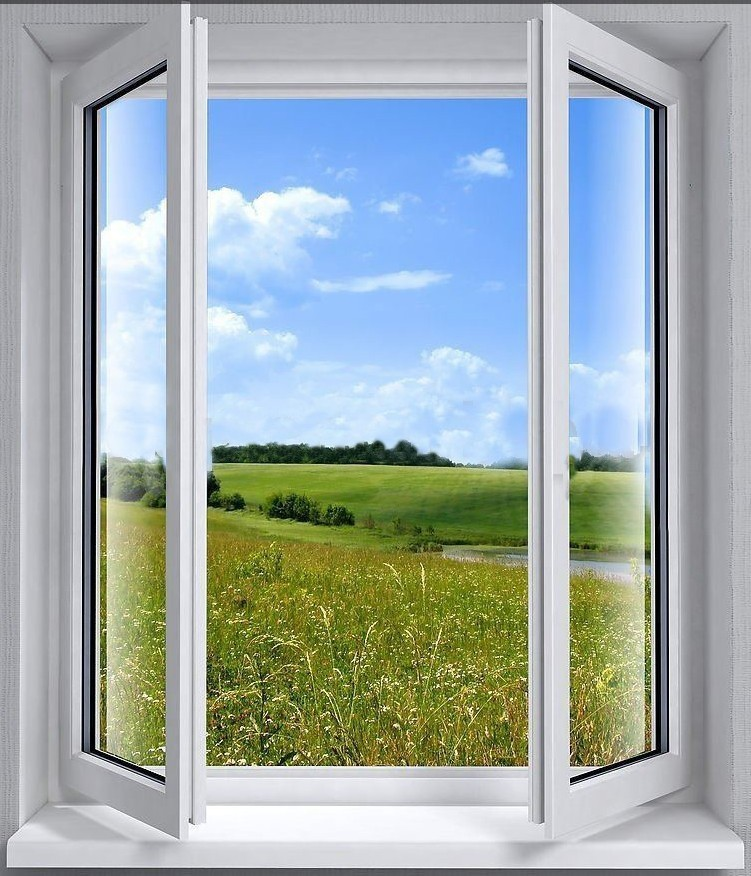
\includegraphics[width=5cm]{c0.windows.view.02.jpg}}
    \quad
    \visible<2->{
\includegraphics[width=5.4cm]{c0.linux.view.02.png}}
  \end{figure}
\end{frame}

\begin{frame}
  \frametitle{Linux的世界}
  \begin{figure}
    \centering
    %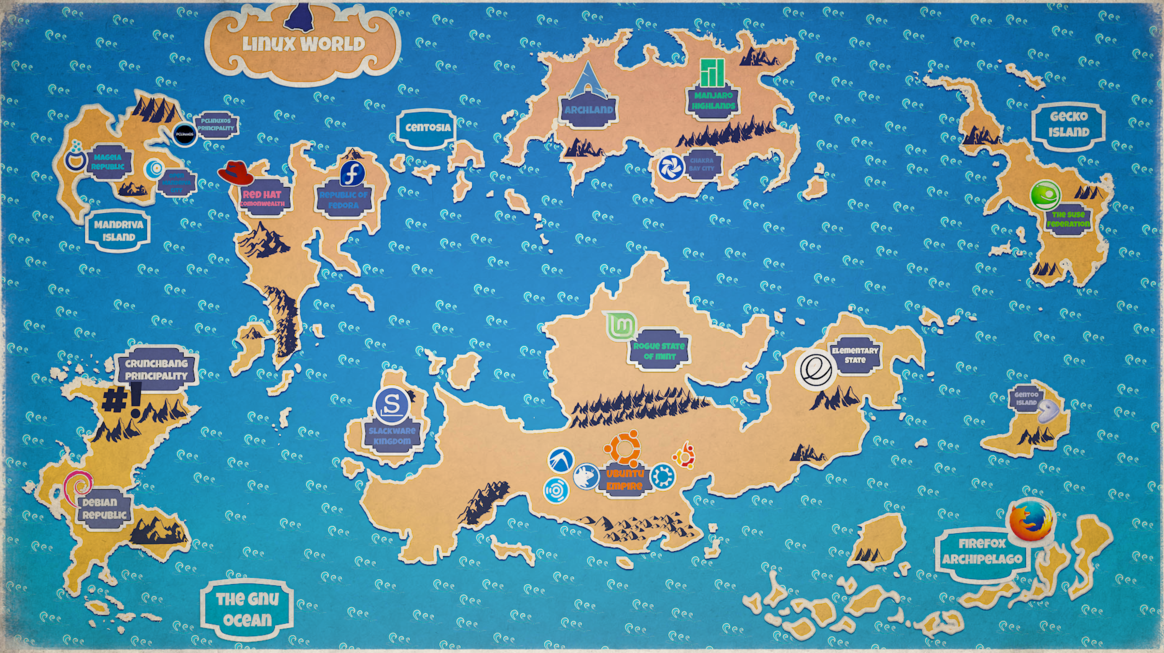
\includegraphics[width=12cm]{c0.linux.world.04.png}
    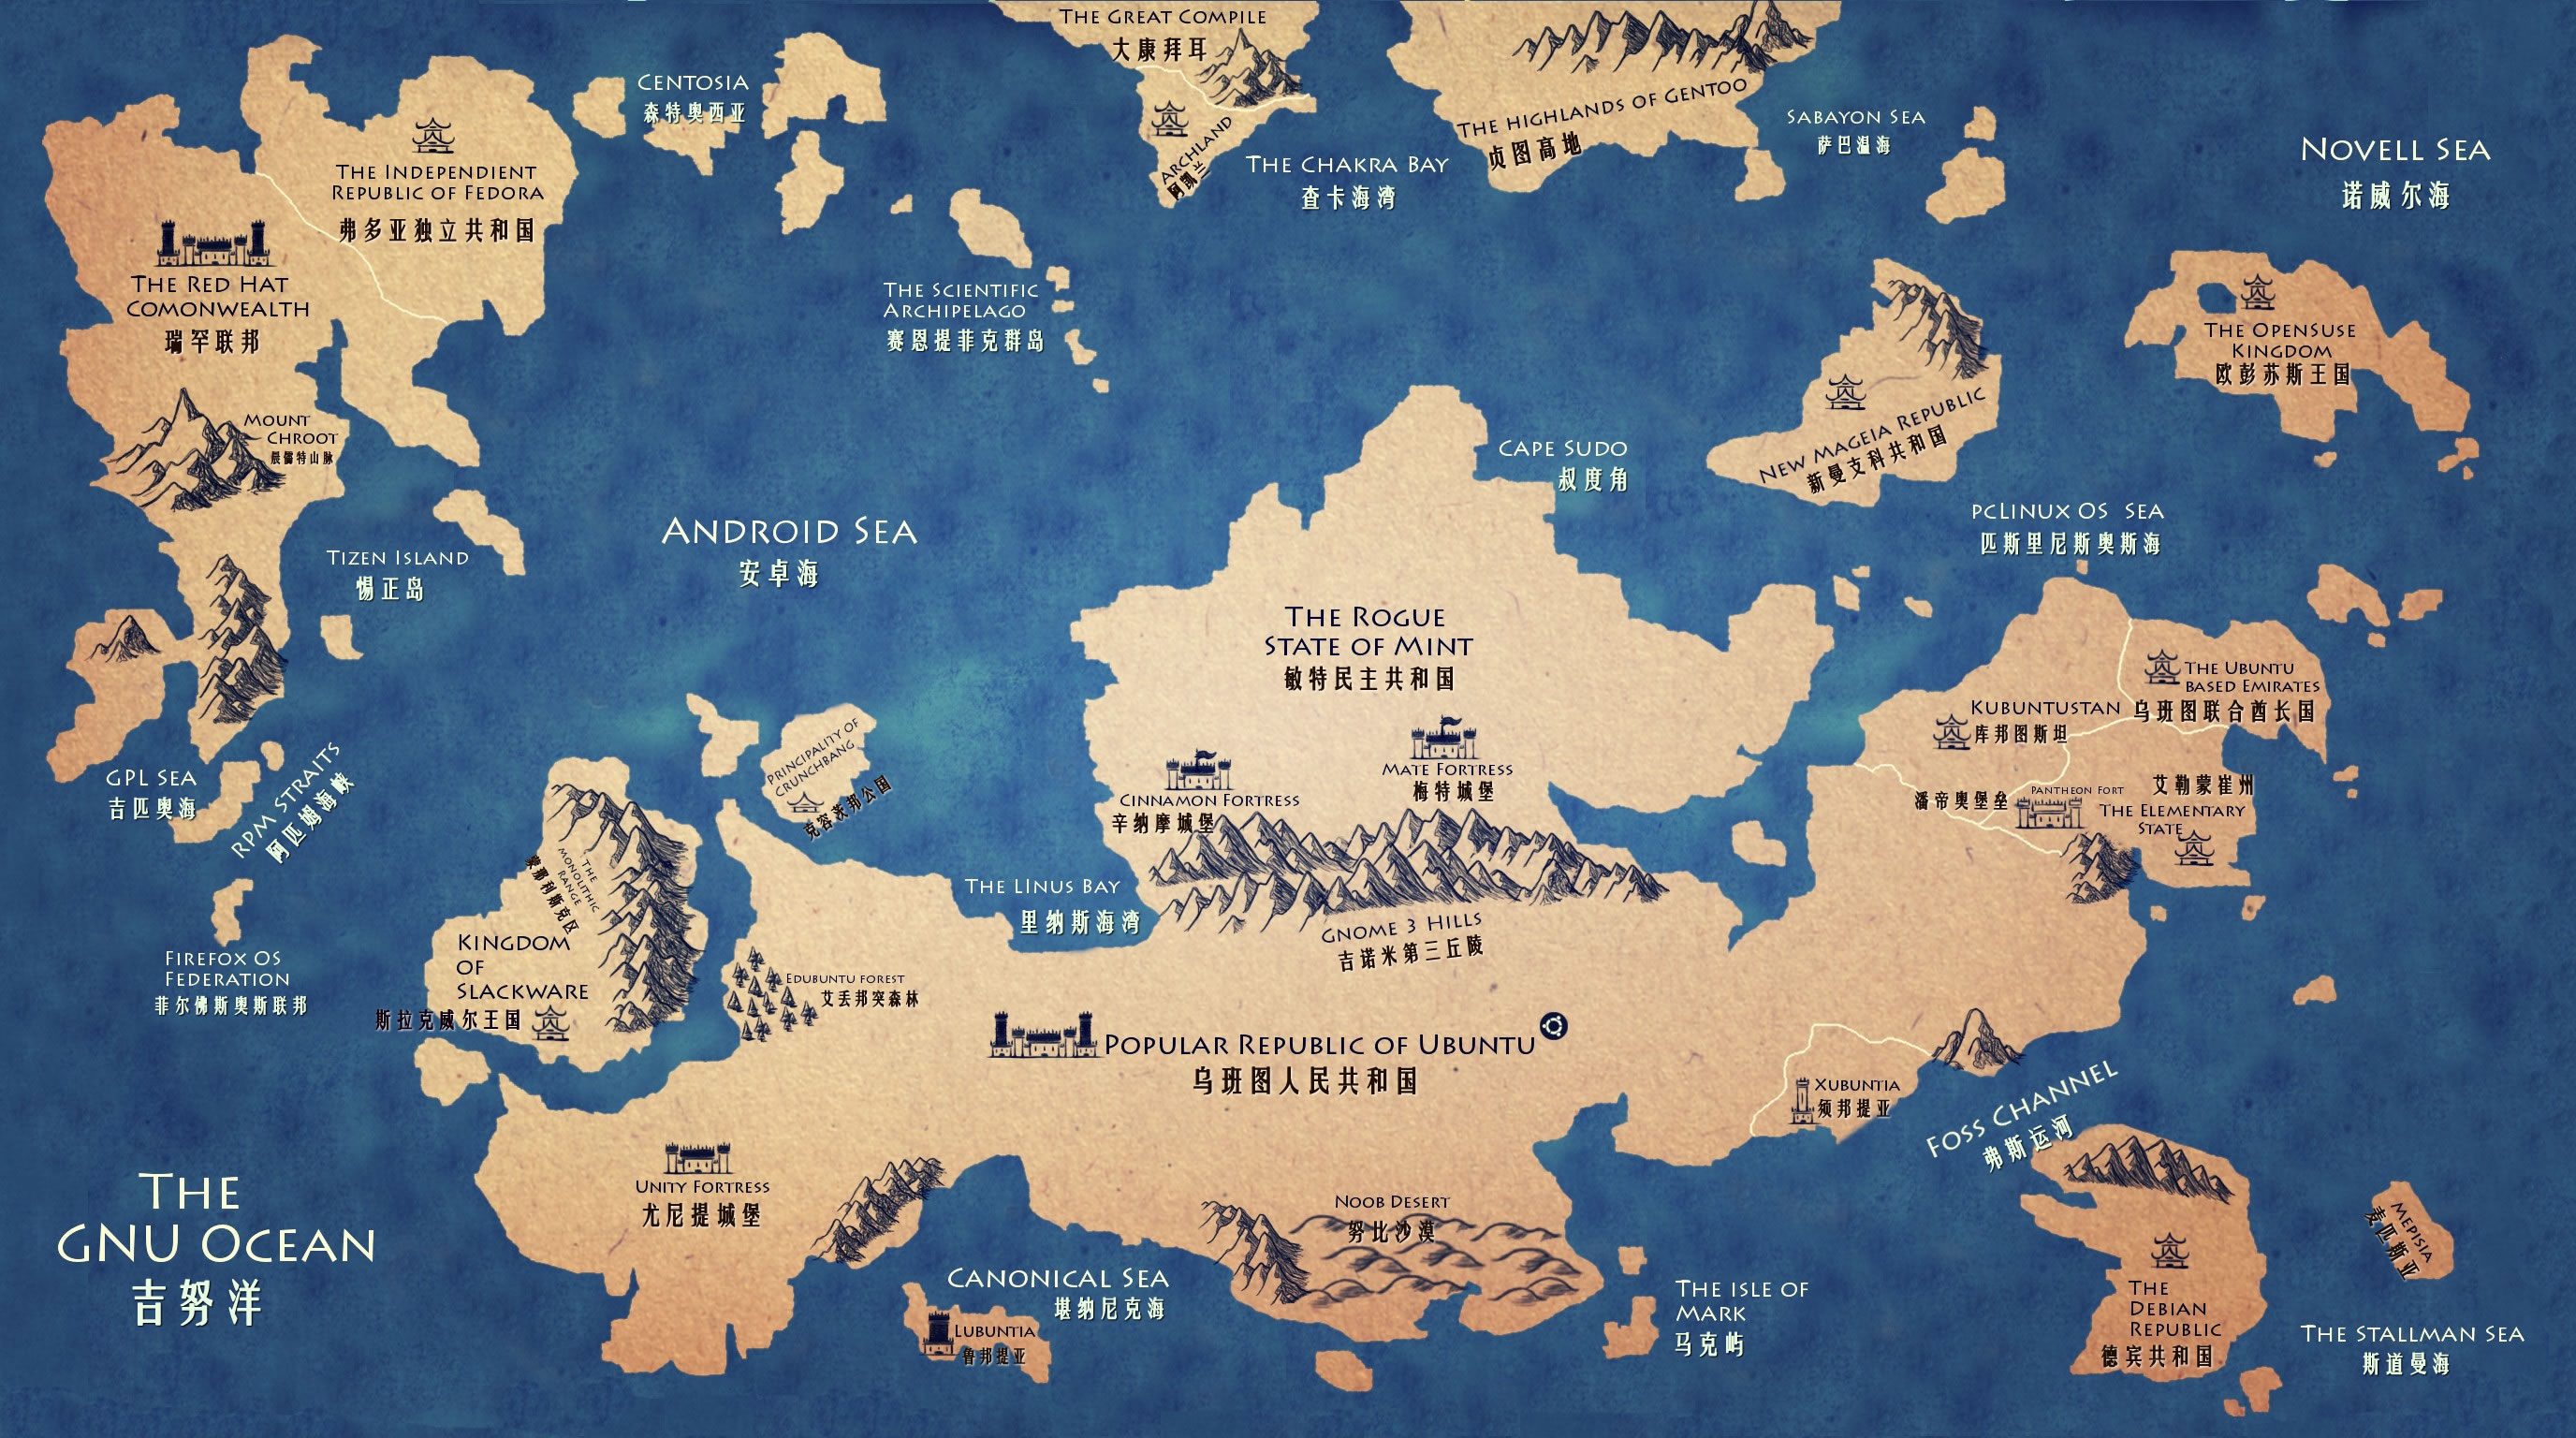
\includegraphics[width=12cm]{c0.linux.world.06.jpg}
  \end{figure}
\end{frame}

\begin{frame}
  \frametitle{授课教材}
  \begin{figure}
    \centering
    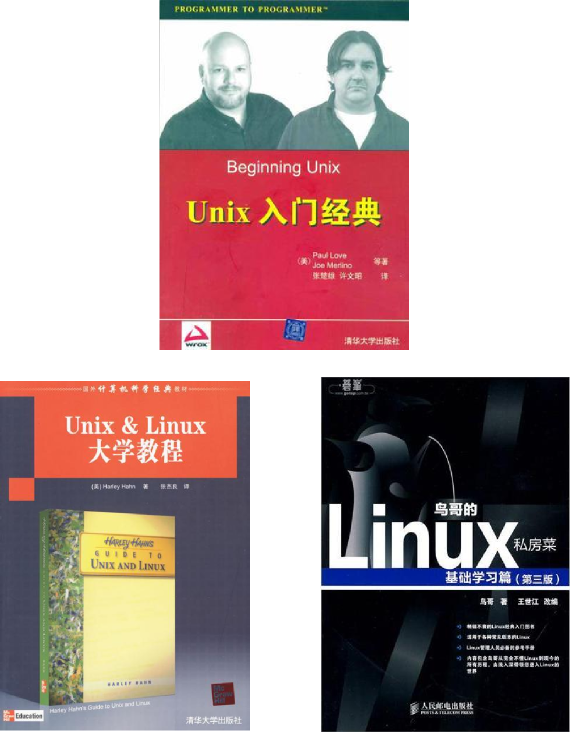
\includegraphics[width=6cm]{c0.books.png}
  \end{figure}
\end{frame}

\begin{frame}
  \frametitle{课程安排 | 理论课}
  \begin{center}
  \alert{前9周,每周三,上午前两节(8:00-9:50),西楼608}\\
  \vspace{0.2cm}
  {\footnotesize
  \textit{纯英文的幻灯片大部分摘抄自edX上的课程:\\ \href{https://www.edx.org/course/introduction-linux-linuxfoundationx-lfs101x-2}{LinuxFoundationX: LFS101x.2 Introduction to Linux}}
  }
  \end{center}
  \vspace{-0.5cm}
  \begin{table}
    \centering
    \rowcolors[]{1}{blue!20}{blue!10}
    \begin{tabular}{cllcc}
      \hline
      \rowcolor{blue!50}顺序 & 授课内容 & 教材章节 & 学时 & 日期\\
      \hline
      1 & Linux基础 & 第1、2章 & 2 & 3.2\\
      2 & 用户和组 & 第3章 & 2 & 3.9\\
      3 & 文件系统 & 第4章 & 2 & 3.16\\
      4 & Linux命令 & 第6章 & 2 & 3.23\\
      5 & 高级Linux命令 & 第8、9章 & 2 & 3.30\\
      6 & 软件安装 & 第19章 & 2 & 4.6\\
      7 & vi/Vim编辑器 & 第7章 & 2 & 4.13\\
      8 & shell脚本编程(上) & 第13、14章 & 2 & 4.20\\
      9 & shell脚本编程(下) & 第13、14章 & 2 & 4.27\\
      %9 & Perl语言简介 & 第17章 & 2 & 7.07\\
      \hline
    \end{tabular}
  \end{table}
\end{frame}

\begin{frame}
  \frametitle{课程安排 | 实验课}
  \begin{center}
  \alert{前9周,每周三,下午前两节(13:30-15:20),教一楼304}\\
  \vspace{0.2cm}
  {\footnotesize
  \textit{部分实验内容摘抄自:\\ 《Linux基础及应用习题解析与实验指导》(谢蓉\ 编著,第二版,中国铁道出版社)}
  }
  \end{center}
  \vspace{-0.5cm}
  \begin{table}
    \centering
    \rowcolors[]{1}{blue!20}{blue!10}
    \begin{tabular}{cllcc}
      \hline
      \rowcolor{blue!50}顺序 & 实验内容 & 理论知识 & 学时 & 日期\\
      1 & 在虚拟机中安装Linux & Linux基础 & 2 & 3.2\\
      2 & Linux图形界面下的文件操作 & \textcolor{gray}{文件系统} & 2 & 3.9\\
      3 & Linux命令行下的文件操作 & 文件系统 & 2 & 3.16\\
      4 & Linux常用命令操作 & Linux命令 & 2 & 3.23\\
      5 & Linux高级命令操作 & 高级Linux命令 & 2 & 3.30\\
      6 & Linux中软件的安装 & 软件安装 & 2 & 4.6\\
      7 & Vim编辑器的使用 & vi/Vim编辑器 & 2 & 4.13\\
      8 & shell脚本的编写(上) & shell脚本编程(上) & 2 & 4.20\\
      9 & shell脚本的编写(下) & shell脚本编程(下) & 2 & 4.27\\
      %9 & Perl脚本的编写 & Perl语言简介 & 2 & 7.09\\
      \hline
    \end{tabular}
  \end{table}
\end{frame}

\begin{frame}
  \frametitle{考核方式}
  \begin{enumerate}
    \item 理论课:60\%
      \begin{enumerate}
        \item 平时表现:10\%
        \item 闭卷考试:50\%
      \end{enumerate}
    \item 实验课:40\%
      \begin{enumerate}
        \item 平时表现:20\%
        \item 实验报告:20\%
      \end{enumerate}
  \end{enumerate}
\end{frame}



\begin{frame}
  \titlepage
\end{frame}

\begin{frame}[plain]
  \frametitle{教学提纲}
  \setcounter{tocdepth}{3}
  \begin{multicols}{2}
    \tableofcontents
  \end{multicols}
\end{frame}

\section{引言}
\begin{frame}
  \frametitle{Linux基础 | 引言 | 操作系统}
  \begin{figure}
    \centering
    
\includegraphics[width=10cm]{c1.os.01.jpg}
  \end{figure}
\end{frame}

\begin{frame}
  \frametitle{Linux基础 | 引言 | 操作系统}
  \begin{figure}
    \centering
    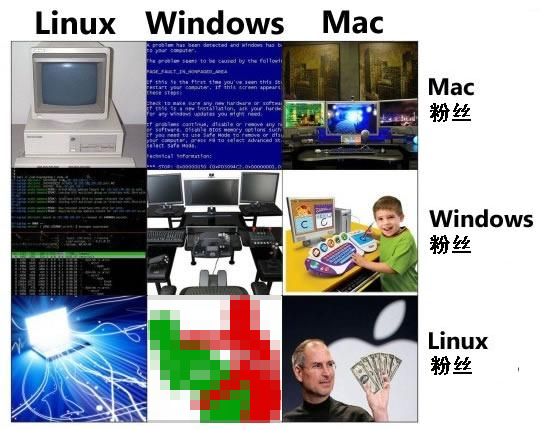
\includegraphics[width=10cm]{c1.os.vs.01.png}
  \end{figure}
\end{frame}

\begin{frame}
  \frametitle{Linux基础 | 引言 | 操作系统}
  \begin{quotation}
    The fundamental difference between Unix and the Macintosh operating system is that \textcolor{magenta}{Unix} was designed to please \textcolor{magenta}{programmers}, whereas the \textcolor{green}{Mac} was designed to please \textcolor{green}{users}. (\textcolor{blue}{Windows}, on the other hand, was designed to please \textcolor{blue}{accountants}, but that's another story.)
    \begin{flushright}
      ——\textit{The Unix-Haters Handbook}\\《Unix痛恨者手册》
    \end{flushright}
  \end{quotation}
\end{frame}

\section{Linux简介}
\subsection{发展简史}
\begin{frame}
  \frametitle{Linux基础 | 简介 | 历史 | Unix进化史}
  \begin{figure}
    \centering
    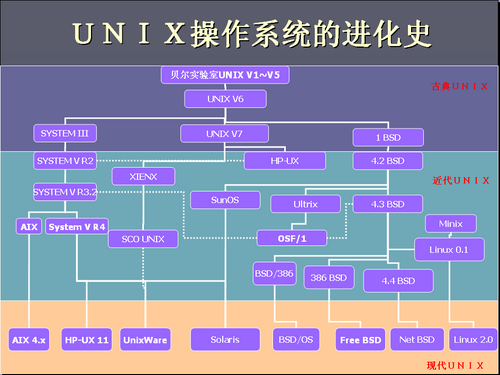
\includegraphics[width=10cm]{c1.unix.history.png}
  \end{figure}
\end{frame}

\begin{frame}
  \frametitle{Linux基础 | 简介 | 历史 | 概述}
  \begin{description}
    \item[燃烧的长江] 20世纪60年代末~80年代初:Unix帝国的崛起、繁荣与分裂
    \item[英雄的黎明] 20世纪80年代:黎明前的黑暗——只为等待Linux的诞生
    \item[辽阔的大地] 20世纪90年代~至今:Linux帝国的诞生与成长
  \end{description}
  \begin{figure}
    \centering
    \visible<2->{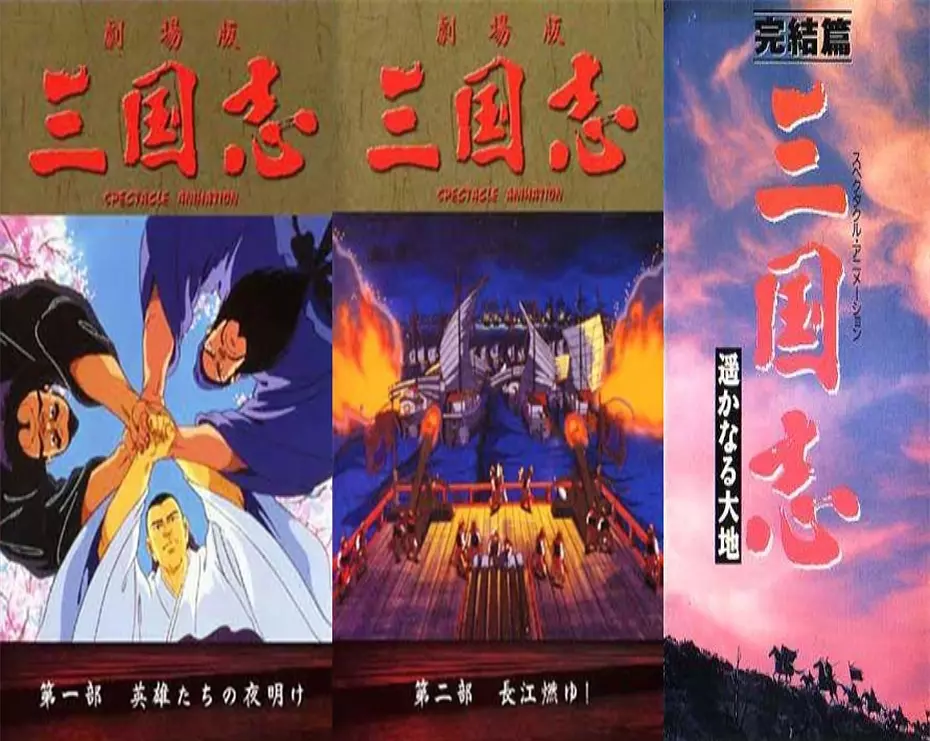
\includegraphics[height=0.55\textheight,width=0.9\textwidth]{c1.history.sanguo.png}}
  \end{figure}
\end{frame}

\begin{frame}
  \frametitle{Linux基础 | 简介 | 历史 | Unix简史}
  \begin{columns}
    \column{0.7\textwidth}
  %\begin{itemize}[<+-|alert@+>]
  \begin{itemize}[<+->]
%\parpic[fr]{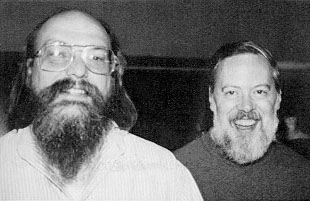
\includegraphics[width=2cm]{c1.tr.jpg}}
%\parpic[fr]{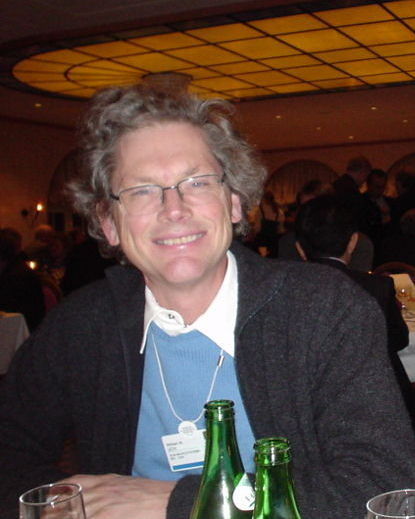
\includegraphics[width=2cm]{c1.joy.jpg}}
    \item 1960s,贝尔实验室(属于AT\&T公司)、通用电气(GE)和麻省理工学院(MIT),Multics
    \item 1969,Ken Thompson(肯\textbullet 汤普逊),贝尔实验室,Unics $\Rightarrow$ Unix
    \item 1973,\alert{Ken Thompson \& Dennis Ritchie}(丹尼斯\textbullet 里奇),用C语言重写\alert{Unix}
    \item 1974,Ken Thompson \& Dennis Ritchie,The UNIX Time-Sharing System(\textit{Communications of the ACM})
    \item 1977,Bill Joy(比尔\textbullet 乔依),加利福尼亚大学伯克利分校,BSD(Berkeley Software Distribution)
    \item 1979,AT\&T公司收回Unix版权,1982:Unix System III $\Rightarrow$ 1983:System V
  \end{itemize}
    \column{0.3\textwidth}
    \visible<2->{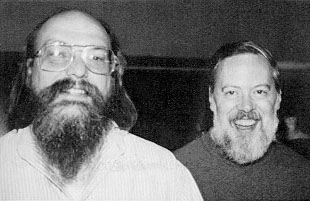
\includegraphics[width=\textwidth]{c1.tr.jpg}}
    \vspace{0.2cm}
    \visible<5->{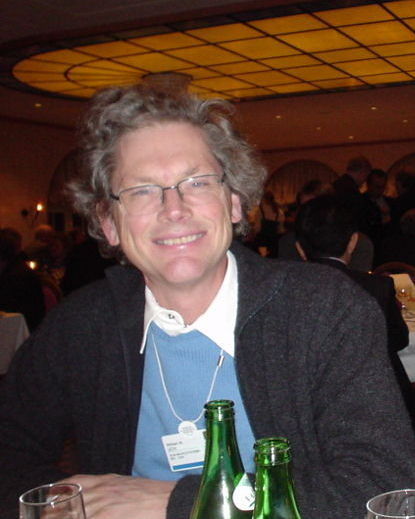
\includegraphics[width=\textwidth]{c1.joy.jpg}}
  \end{columns}
\end{frame}

\begin{frame}
  \frametitle{Linux基础 | 简介 | 历史 | Linux简史}
  \begin{columns}
    \column{0.78\textwidth}
  %\begin{itemize}[<+-|alert@+>]
  \begin{itemize}[<+->]
    \item 1983,\alert{Richard Stallman}(理查德\textbullet 斯托曼),\alert{GNU(GNU's Not Unix)}计划:希望发展出一套完整的开放源代码操作系统来取代Unix
    \item 1985,Richard Stallman,自由软件基金会(Free Software Foundation,FSF):执行GNU计划,开发更多的自由软件
    \item 1985,Richard Stallman,GNU宣言:解释和定义GNU计划的目标,并呼吁人们参与及支持,是自由软件运动的核心精神
    \item 1989,Richard Stallman,GNU通用公共许可协议(GNU General Public License,\alert{GPL}),非盈利版权(Copyleft)
    \item 源于1985,POSIX(便携式操作系统界面,Portable Operating Systems Interface)标准,适用于所有Unix版本的综合标准
  \end{itemize}
    \column{0.2\textwidth}
    \visible<1->{
\includegraphics[width=\textwidth]{c1.stallman.01.jpg}}
    \visible<1->{
\includegraphics[width=\textwidth]{c1.gnu.png}}
    %\vspace{0.05cm}
    %\visible<3->{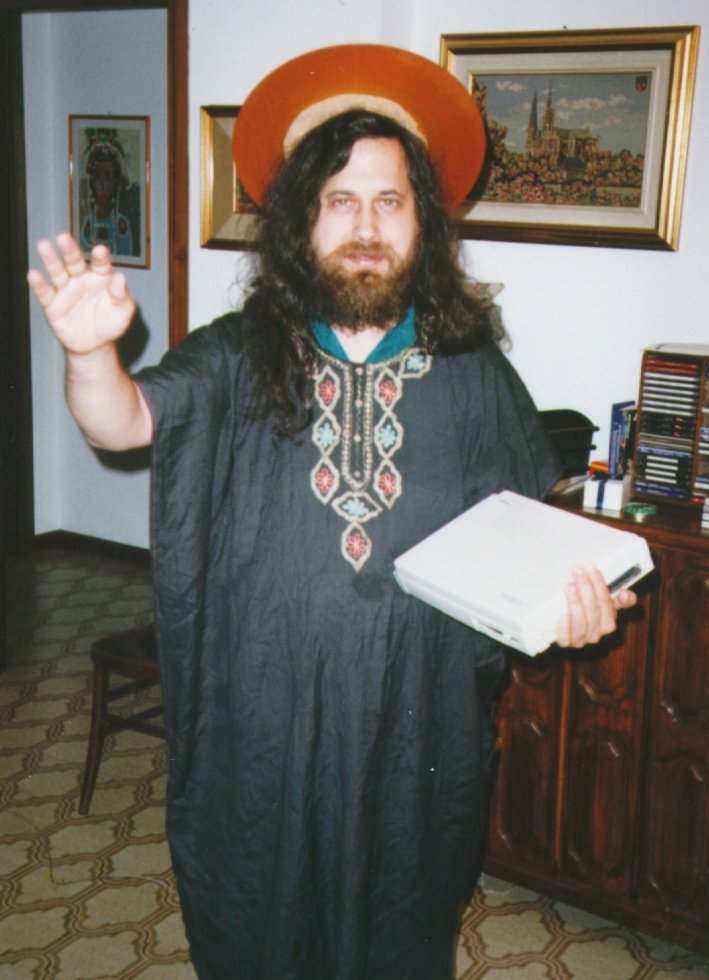
\includegraphics[width=\textwidth]{c1.stallman.03.jpg}}
    \visible<4->{
\includegraphics[width=\textwidth]{c1.stallman.02.jpg}}
    %\vspace{0.05cm}
  \end{columns}
\end{frame}

\begin{frame}
  \frametitle{Linux基础 | 简介 | 历史 | Linux简史(续)}
  \begin{columns}
    \column{0.78\textwidth}
  %\begin{itemize}[<+-|alert@+>]
  \begin{itemize}[<+->]
    \item 1987,Andrew Tanenbaum(安德鲁\textbullet 谭宁邦),荷兰阿姆斯特丹自由大学,Minix
    \item 1990,FSF,Hurd:GNU操作系统的微内核
    \item 1991,\alert{Linus Torvalds}(李/林纳斯\textbullet 托瓦兹),芬兰赫尔辛基大学,Freax$\rightarrow$ \alert{Linux}(类Unix系统,Unix-like)
    \item 1992,在GNU GPL下Linux内核被重新授权使用
    \item 1993,Slackware首次发布;Debian项目设立
    \item 1994,Linux内核1.0版本发布
    \item 1996,Linux内核2.0版本发布
    \item 2011,Linux内核3.0版本发布
    \item 2015,Linux内核4.0版本发布
    \item GNU项目软件 + Linux内核 = \alert{GNU/Linux}
  \end{itemize}
    \column{0.22\textwidth}
    %\visible<1->{\includegraphics[width=\textwidth]{c1.stallman.11.jpg}}
    %\vspace{0.05cm}
    \visible<1->{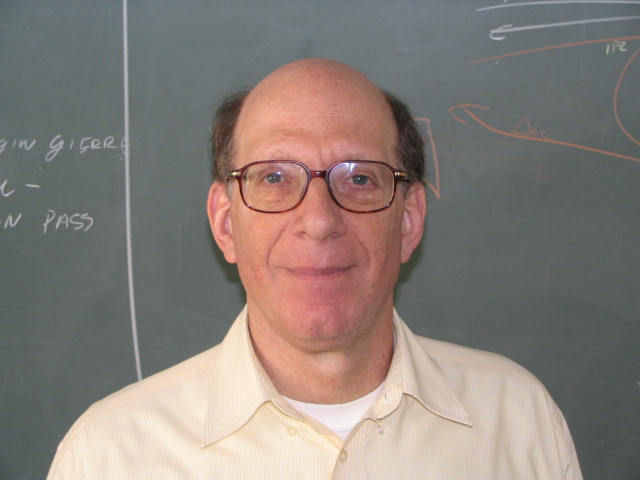
\includegraphics[width=\textwidth]{c1.tanenbaum.png}}
    %\vspace{0.05cm}
    \visible<3->{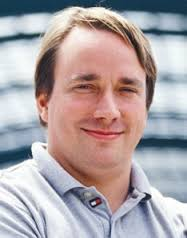
\includegraphics[width=\textwidth]{c1.torvalds.jpg}}
  \end{columns}
\end{frame}

\begin{frame}
  \frametitle{Linux基础 | 简介 | 历史 | 拾遗}
  \begin{columns}
    \column{0.8\textwidth}
  %\begin{itemize}[<+-|alert@+>]
  \begin{itemize}[<+->]
    \item 1980,Tim Paterson(蒂姆\textbullet 帕特森),86-DOS
    \item 1981,微软公司收购86-DOS,更名为MS-DOS
    \item 1984,苹果公司,System 1.0
    \item 1985,微软公司,Windows 1.0
    \item 1993,Patrick Volkerding,Slackware(现存最古老的Linux发行版)
    \item 1995,Red Hat(红帽公司)成立;1999年上市
    \item 1996,Larry Ewing(拉里\textbullet 厄文),设计创作了Linux吉祥物——\alert{Tux}
    % \item 2001,苹果公司,Mac OS X/OS X/macOS = Darwin(Mach内核 + BSD实现)+ Aqua界面
    \item 2001,苹果公司,Mac OS X/OS X/macOS
    \item 2004,Canonical公司(科能软件有限公司)成立(Ubuntu家族的Linux发行版)
    \item 2007,Google发布Android的源代码(Apache)
    \item 2008,第一部Android智能手机发布
  \end{itemize}
    \column{0.2\textwidth}
    \visible<7->{
\includegraphics[width=\textwidth]{c1.tux.png}}
    %\vspace{0.5cm}
    \visible<10->{
\includegraphics[width=\textwidth]{c1.android.png}}
  \end{columns}
\end{frame}

\begin{frame}
  \frametitle{Linux基础 | 简介 | 历史 | 20周年}
  \begin{figure}
    \centering
    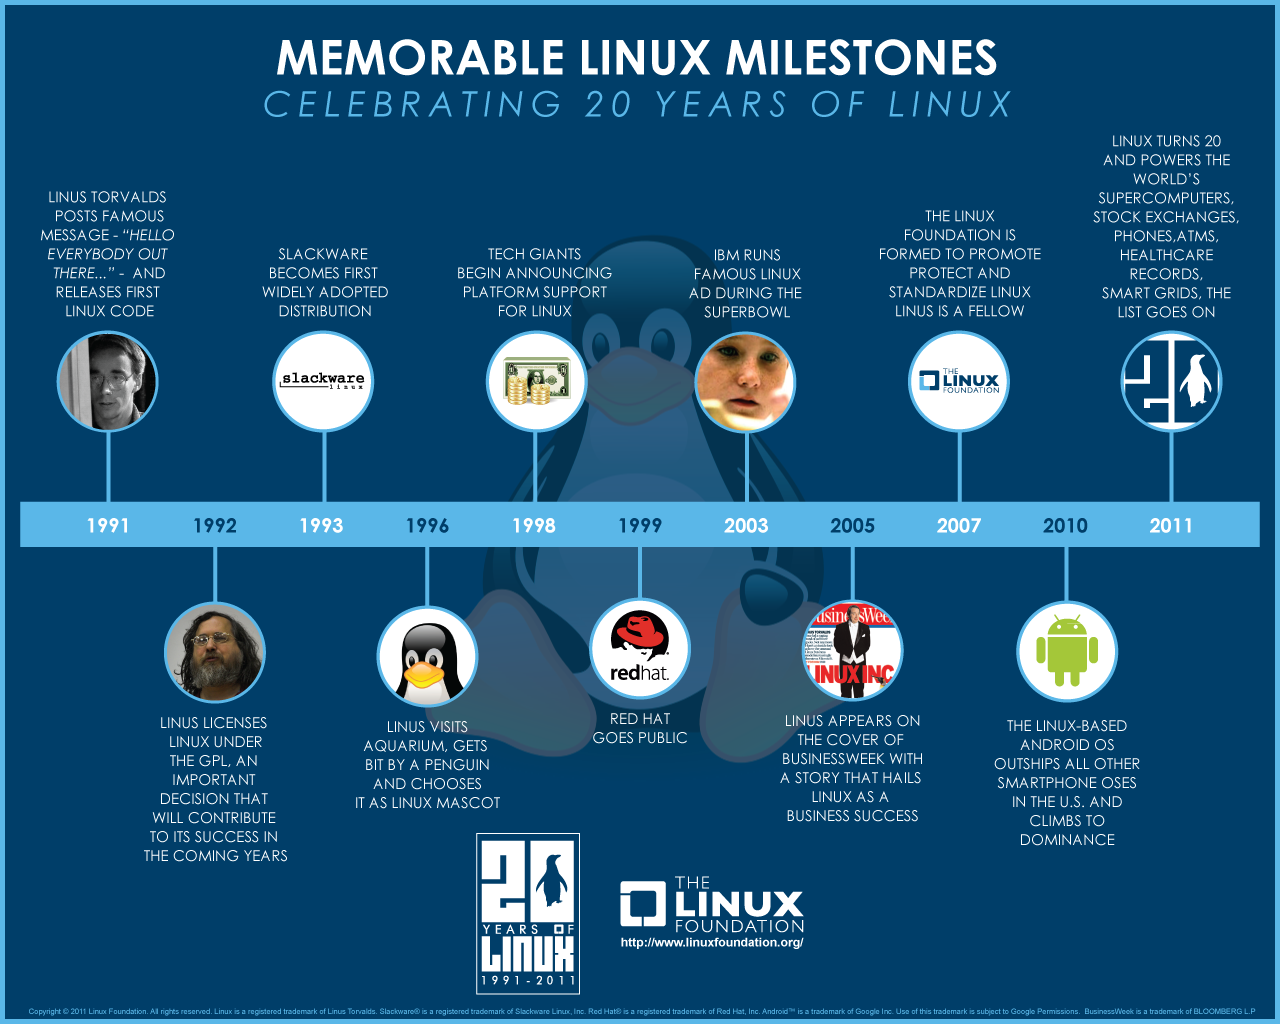
\includegraphics[width=12cm,height=7cm]{c1.linux.history.png}
  \end{figure}
\end{frame}

\begin{frame}
  \frametitle{Linux基础 | 简介 | 发音}
  \begin{block}{Linux的发音}
  根据托瓦兹的说法,Linux的发音和“Minix”是押韵的。“Li”中“i”的发音类似于“Minix”中“i”的发音,而“nux”中“u”的发音类似于英文单词“profess”中“o”的发音。依照国际音标应该是\begin{IPA}[tt]['lIn@ks]\end{IPA}。
  \end{block}
  \pause
  \begin{block}{词典中的注音}
    \begin{description}
      \item[有道词典] \begin{IPA}[tt]['lIn@ks]\end{IPA}
      \item[金山词霸] \begin{IPA}[tt]['lIn@ks]\end{IPA}(UK); \begin{IPA}[tt]['lIn@ks]\end{IPA}(US)
      \item[必应词典] \begin{IPA}[tt]['lIn@ks]\end{IPA}(UK); \begin{IPA}[tt]['laIn2ks]\end{IPA}(US)
      \item[欧路词典] \begin{IPA}[tt]['laIn2ks]\end{IPA}
    \end{description}
  \end{block}
  \pause
  \begin{block}{Linux读Linux}
    ``Hello, this is Linus Torvalds, and I pronounce Linux as Linux''.
  \end{block}
\end{frame}

\begin{frame}
  \frametitle{Linux基础 | 简介 | 发音}
  \begin{figure}
    \centering
    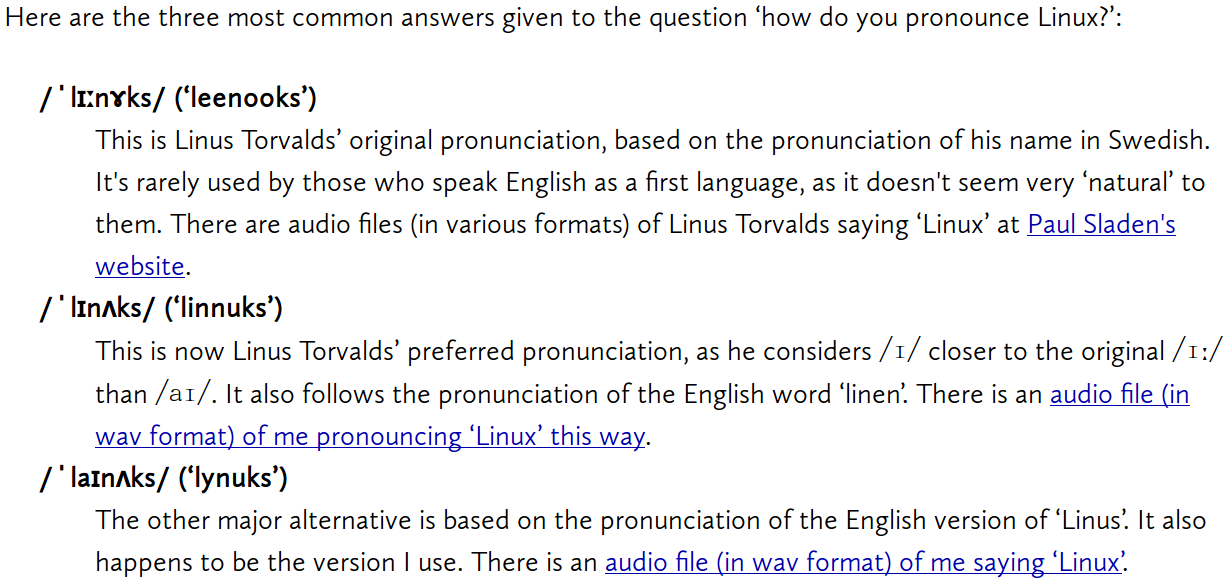
\includegraphics[width=12cm]{c1.linux.pronunciation.png}
  \end{figure}
\end{frame}

\subsection{Linux操作系统}
\begin{frame}
  \frametitle{Linux基础 | 简介 | Linux系统 | Linux}
  \begin{block}{\alert{Linux的两层含义}}
    \begin{enumerate}
      \item Linux内核
      \item 基于Linux内核的操作系统
    \end{enumerate}
  \end{block}
  \pause
  \begin{block}{Linux内核}
    \begin{itemize}
      \item 操作系统最底层的内核及其提供的内核工具
      \item GNU GPL授权模式
      \item 参考POSIX设计规范,兼容于Unix操作系统
    \end{itemize}
  \end{block}
  \pause
  \begin{block}{\alert{Linux操作系统}}
    \begin{itemize}
      \item 一种多用户、多任务处理的类Unix操作系统
      \item 由Linux内核、shell和实用工具等构成
    \end{itemize}
  \end{block}
\end{frame}

\begin{frame}
  \frametitle{Linux基础 | 简介 | Linux系统 | 特色}
  \begin{itemize}
    \item 自由与开放的使用与学习环境
    \item 配备需求低廉
    \item 内核功能强大而稳定
    \item 独立作业
  \end{itemize}
\end{frame}

\begin{frame}
  \frametitle{Linux基础 | 简介 | Linux系统 | 优点}
  \begin{itemize}
    \item 优良的稳定性和安全性,漏洞的快速修补
    \item 免费或少许费用,大量的可用软件和免费软件
    \item 多任务、多用户,用户与用户组的规划
    \item 良好的可移植性和灵活性,相对比较不耗资源,适合需要小内核程序的嵌入式系统
    \item 整合度佳且多样的图形用户界面(GUI)
    \item 多数网络协议支持,方便的远程管理
    \item 强大的内存管理和文件管理系统
    \item ……
  \end{itemize}
\end{frame}

\begin{frame}
  \frametitle{Linux基础 | 简介 | Linux系统 | 缺点}
  \begin{itemize}
    \item 没有特定的支持厂商
    \item 游戏的支持度不高
    \item 专业软件的支持度不足
  \end{itemize}
\end{frame}

\subsection{Linux发行版}
\begin{frame}
  \frametitle{Linux基础 | 简介 | 发行版 | vs. 品牌机}
  \begin{block}{品牌机}
    由公司性质组装起来的电脑,并且经过兼容性测试,而正式对外出售的整套的电脑。
  \end{block}
  \begin{figure}
    \centering
    
\includegraphics[width=0.5\textwidth]{c1.pinpai.computer.01.jpg}
    
\includegraphics[width=0.45\textwidth]{c1.pinpai.mobile.png}
  \end{figure}
\end{frame}

\begin{frame}
  \frametitle{Linux基础 | 简介 | 发行版}
  \begin{block}{Linux发行版}
    Linux distributions是“Linux Kernel + Free Software + Documentations(Tools) + 可完全安装的程序”所制成的一套完整的系统。
    \begin{itemize}
      \item Linux内核
      \item 实用工具
      \item 编程工具
      \item 至少一个GUI
    \end{itemize}
  \end{block}
  \pause
  \begin{figure}
    \centering
    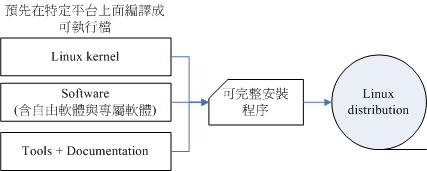
\includegraphics[width=8cm]{c1.linux.distribution.01.png}
  \end{figure}
\end{frame}

\begin{frame}
  \frametitle{Linux基础 | 简介 | 发行版}
  \begin{figure}
    \centering
    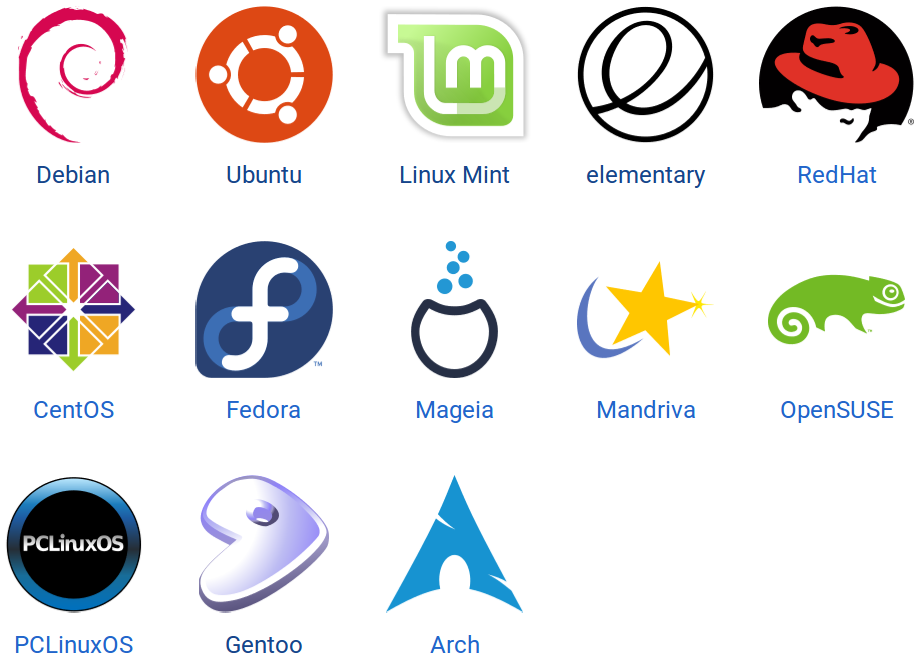
\includegraphics[width=10cm]{c1.linux.distribution.03.png}
  \end{figure}
\end{frame}

\begin{frame}
  \frametitle{Linux基础 | 简介 | 发行版}
  \begin{figure}
    \centering
    
\includegraphics[width=12cm]{c1.linux.distribution.02.png}
  \end{figure}
\end{frame}

\begin{frame}
  \frametitle{Linux基础 | 简介 | 发行版 | \alert{两大系统}}
  \begin{enumerate}
    \item Red Hat系(基于RPM软件包管理系统)
      \begin{itemize}
        \item Red Hat Enterprise Linux(RHEL)
        \item CentOS
        \item Fedora
        \item SUSE/openSUSE
      \end{itemize}
    \item Debian系(基于dpkg软件包管理系统)
      \begin{itemize}
        \item Debian
        \item Ubuntu
        \item Linux Mint
        \item Deepin
      \end{itemize}
  \end{enumerate}
\end{frame}

\begin{frame}
  \frametitle{Linux基础 | 简介 | 发行版 | \alert{三大家族}}
  \begin{figure}
    \centering
    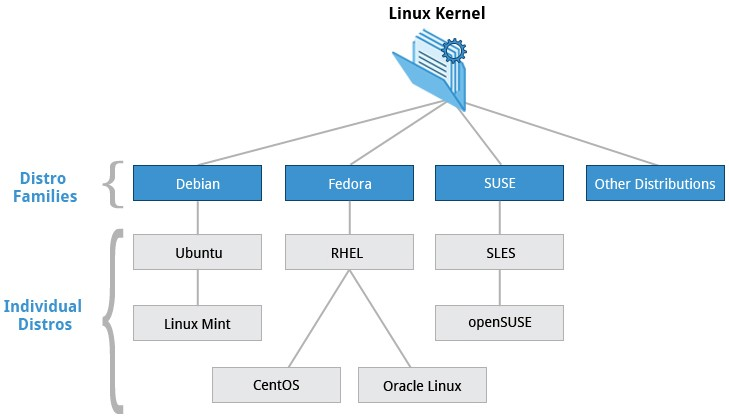
\includegraphics[width=11cm]{c1.distribution.family.01.jpg}
  \end{figure}
\end{frame}

\begin{frame}
  \frametitle{Linux基础 | 简介 | 发行版 | \alert{三大家族}}
  \begin{columns}
    \column{0.3\textwidth}
    \begin{block}{Fedora: RPM, Yum}
      \begin{figure}
        \centering
        
\includegraphics[width=2.3cm]{distribution.logos/rhel.01.jpg}\\
        
\includegraphics[width=2.3cm]{distribution.logos/centos.01.png}\\
        
\includegraphics[width=2.3cm]{distribution.logos/fedora.01.jpg}
      \end{figure}
    \end{block}
    \column{0.3\textwidth}
    \begin{block}{Debian: dpkg, APT}
      \begin{figure}
        \centering
        
\includegraphics[width=2.2cm]{distribution.logos/debian.01.png}\\
        
\includegraphics[width=2.2cm]{distribution.logos/ubuntu.01.jpg}\\
        
\includegraphics[width=2.2cm]{distribution.logos/mint.01.png}
      \end{figure}
    \end{block}
    \column{0.32\textwidth}
    \begin{block}{SUSE: RPM, Zypper}
      \begin{figure}
        \centering
        
\includegraphics[width=3.5cm]{distribution.logos/suse.01.jpg}\\
	\vspace{0.5cm}
        
\includegraphics[width=3.5cm]{distribution.logos/opensuse.01.jpg}
      \end{figure}
    \end{block}
  \end{columns}
\end{frame}

\begin{frame}
  \frametitle{Linux基础 | 简介 | 发行版 | \alert{三大家族}}
  \begin{figure}
    \centering
    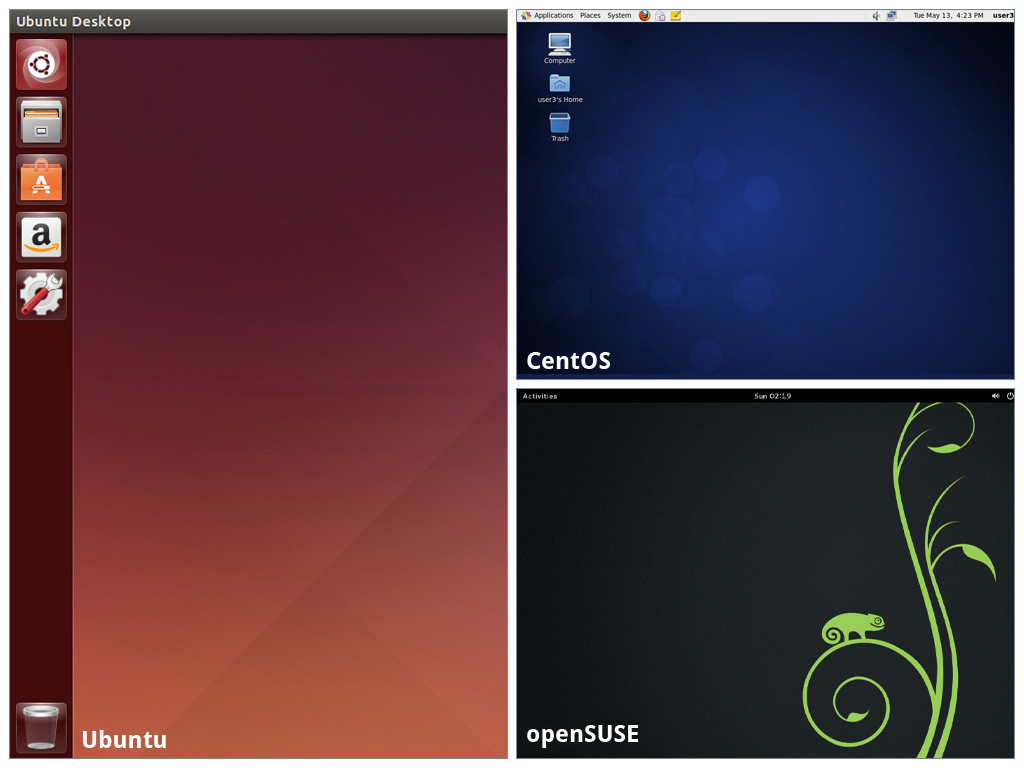
\includegraphics[width=12cm,height=7.5cm]{c1.ubuntu.centos.opensuse.jpg}
  \end{figure}
\end{frame}

\begin{frame}
  \frametitle{Linux基础 | 简介 | 发行版 | 桌面环境}
  \begin{block}{桌面环境}
    一个桌面环境(Desktop environment,有时称为桌面管理器)为计算机提供一个图形用户界面(GUI)。这个名称来自桌面比拟,对应于早期的文字命令行界面(CLI)。一个典型的桌面环境提供图标、视窗、工具栏、文件夹、壁纸以及像拖放这样的能力。整体而言,桌面环境在设计和功能上的特性,赋予了它与众不同的外观和感觉。
  \end{block}
  \pause
  \begin{block}{Windows \& Mac}
    流行的私有操作系统Microsoft Windows和Mac OS X所用的桌面环境是相对不可变的。但是也有主题和第三方软件可以完全更改常见界面元素的外观(比如窗口、按钮和图标)以及界面本身。
  \end{block}
\end{frame}

\begin{frame}
  \frametitle{Linux基础 | 简介 | 发行版 | 桌面环境 | Linux}
  \begin{description}
    \item[GNOME] GNU网络对象模型环境(The GNU Network Object Model Environment),GNU计划的一部分,开放源代码运动的一个重要组成部分。其目标是基于自由软件,为Unix及类Unix系统构造一个功能完善、操作简单以及界面友好的桌面环境。它是GNU计划的正式桌面。
    \item[KDE] 一个国际性的自由软件社区,开发运行在Linux、BSD、Solaris、Microsoft Windows与Mac OS X等平台上的一系列跨平台应用程序。它最著名的产品是Plasma桌面,是许多Linux发布版的默认桌面环境。
    \item[Unity] Canonical公司为GNOME桌面环境所开发的图形用户界面,用于Ubuntu操作系统。Unity在Ubuntu 10.10上网本版中首次推出,最初是为了充分利用上网本有限的屏幕尺寸。不同于GNOME、KDE,Unity并非一个桌面包。Ubuntu 17.04是最后一个预载Unity桌面环境的版本。
  \end{description}
\end{frame}

\begin{frame}
  \frametitle{Linux基础 | 简介 | 发行版 | 桌面环境 | Linux}
  {\footnotesize
  \begin{description}
    \item[CDE] 通用桌面环境(Common Desktop Environment),运行于Unix、基于Motif部件工具箱开发的商业桌面环境。
    \item[Xfce] 一个在Unix与Unix-like操作系统上运行的桌面环境。Xfce的设计目的是“设计为可作为实际应用,快速加载及运行程序,并减少耗用系统资源”。
    \item[LXDE] Lightweight X11 Desktop Environment,是自由桌面环境,可在Unix以及Linux等POSIX兼容平台运行。LXDE项目旨在提供新的轻量、快速的桌面环境。LXDE重视实用性和轻巧性,并且尽力降低其所耗系统资源。
    \item[Enlightenment] 常简称为E。0.17以前版本属于X窗口管理器,0.17版已经接近完整的桌面环境。而从0.19版开始,同时也是Wayland的合成管理器。
    \item[Cinnamon] Unix-like系统下的一个用户接口。是GNOME Shell的一个派生版本,最初是为Linux Mint所开发,其提供了如同GNOME 2般易于使用的拟真接口。
    \item[MATE] 由已经停止官方维护的GNOME 2源代码派生而来的桌面环境。
    \item[深度桌面环境] Deepin Desktop Environment,基于HTML5和WebKit开发,主要由桌面、启动器、任务栏和深度控制中心组成。除深度控制中心前端使用QML技术,后端使用Go语言编写外,其余部分均为HTML5和WebKit实现。
  \end{description}
  }
\end{frame}

\begin{frame}
  \frametitle{Linux基础 | 简介 | 发行版 | 桌面环境 | Linux}
  \begin{figure}
    \centering
    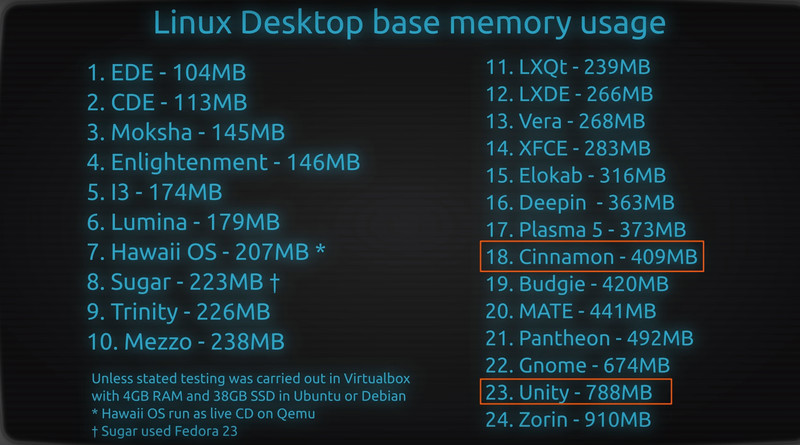
\includegraphics[width=0.9\textwidth]{c1.linux.de.memory.jpg}
  \end{figure}
\end{frame}

\begin{frame}
  \frametitle{Linux基础 | 简介 | \alert{发行版 vs. 桌面环境}}
  \begin{table}
    \centering
    \rowcolors[]{1}{blue!20}{blue!10}
    \begin{tabular}{cl}
      \hline
      \rowcolor{blue!50}桌面环境 & 代表性发行版\\
      \hline
      GNOME & RHEL、CentOS、Fedora、Debian\\
      KDE & openSUSE、Mandriva Linux、Kubuntu\\
      Unity & Ubuntu(11.04~17.04)\\
      Xfce & Xubuntu\\
      LXDE & Lubuntu\\
      Cinnamon & Linux Mint\\
      MATE & Linux Mint\\
      Pantheon & Elementary OS\\
      深度桌面环境 & Deepin\\
      \hline
    \end{tabular}
  \end{table}
\end{frame}

\begin{frame}
  \frametitle{Linux基础 | 简介 | 发行版 | 选择}
  \begin{columns}
    \column{0.45\textwidth}
  \begin{block}{企业环境}
    \begin{itemize}
      \item RHEL
      \item SUSE
    \end{itemize}
  \end{block}
  \pause
  \begin{block}{服务器环境}
    \begin{itemize}
      \item CentOS
      \item openSUSE
      \item Debian
      \item Ubuntu Server
    \end{itemize}
  \end{block}
  \pause
    \column{0.45\textwidth}
  \begin{block}{桌面环境}
    \begin{itemize}
      \item Ubuntu
      \item Linux Mint
      \item Fedora
      \item Deepin
      \item elementary OS
      \item Manjaro Linux
      \item Gentoo
      \item Arch Linux
    \end{itemize}
  \end{block}
\end{columns}
\end{frame}

\begin{frame}
  \frametitle{Linux基础 | 简介 | 发行版 | 2018}
  \begin{block}{2018最佳Linux发行版排行榜}
    \begin{description}
      \item[最适合系统管理员的发行版] Debian GNU/Linux
      \item[最好的服务器发行版] Ubuntu Server
      \item[最好的桌面发行版] elementary OS
      \item[最漂亮的发行版] Pop!\_OS 
      \item[最好的轻量级发行版] Lubuntu
      \item[最年轻的发行版] Nitrux
      \item[发展最快的发行版] Manjaro Linux 
      \item[性能最好的发行版] Clear Linux
      \item[包管理最好的发行版] Arch Linux
      \item[最能证明能力的发行版] Linux From Scratch 8.0
      \item[最好的教育发行版] ezgo Linux 
      \item[最好的物联网发行版] Ubuntu Core
    \end{description}
  \end{block}
\end{frame}

\begin{frame}
  \frametitle{Linux基础 | 简介 | 发行版 | 2018}
  \begin{block}{2018年10大最漂亮的Linux发行版}
    \begin{itemize}
      \item \href{https://elementary.io/}{elementary OS}: 类macOS的外观
      \item \href{https://zorinos.com/}{Zorin OS}: 类Windows界面及操作,Windows用户上手容易
      \item \href{https://neon.kde.org/}{KDE Neon}: 流畅、稳定、漂亮的扁平化桌面
      \item \href{http://www.deepin.com}{Deepin Linux}: 对一些中国软件的良好支持
      \item \href{https://nxos.org/}{Nitrux}: 极度简约的漂亮桌面
      \item \href{http://ferenos.weebly.com/}{feren OS}: 提供Wine,方便运行Windows程序
      \item \href{https://system76.com/pop}{Pop!\_OS}: 新奇的外观,舒缓的视觉外观,眼睛舒服
      \item \href{https://solus-project.com/}{Solus OS}: 增长最快的新发行版之一
      \item \href{https://mauilinux.org/}{Maui Linux}: 够小众,用户数超少
      \item \href{https://www.opensuse.org}{openSUSE}: 主流发行版,用户庞大,社区支持优异
    \end{itemize}
  \end{block}
\end{frame}

\begin{frame}
  \frametitle{Linux基础 | 简介 | 发行版 | 2016(1/2)}
  \begin{block}{2016最佳Linux发行版排行榜}
  \begin{description}
    \item[最好的企业级系统] SLE/RHEL
    \item[最好的服务器操作系统] Debian/CentOS
    \item[最好的台式机操作系统] Linux Mint Cinnamon
    \item[最好的笔记本操作系统] Ubuntu MATE
    \item[最好的旧硬件支持系统] Lubuntu
    \item[最好看的发行版] elementary OS
    \item[最可定制的发行版] Arch Linux
    \item[最好的教育操作系统] ezgo Linux
    \item[最佳新人] Solus
  \end{description}
  \end{block}
\end{frame}

\begin{frame}
  \frametitle{Linux基础 | 简介 | 发行版 | 2016(2/2)}
  \begin{block}{2016最佳Linux发行版排行榜(续)}
  \begin{description}
    \item[最好的回归发行版] openSUSE
    \item[最好的移动操作系统] Plasma Mobile
    \item[最好的云操作系统] Chrome OS
    \item[最好的隐私保护操作系统] Tails
    \item[最好的多媒体制作系统] Ubuntu Studio
    \item[最好的游戏系统] Steam OS
    \item[最好的物联网操纵系统] Snappy Ubuntu Core
    \item[最好的ARM设备发行版] Arch Linux ARM
  \end{description}
  \end{block}
\end{frame}

\begin{frame}
  \frametitle{Linux基础 | 简介 | 发行版 | 总结}
  \begin{figure}
    \centering
    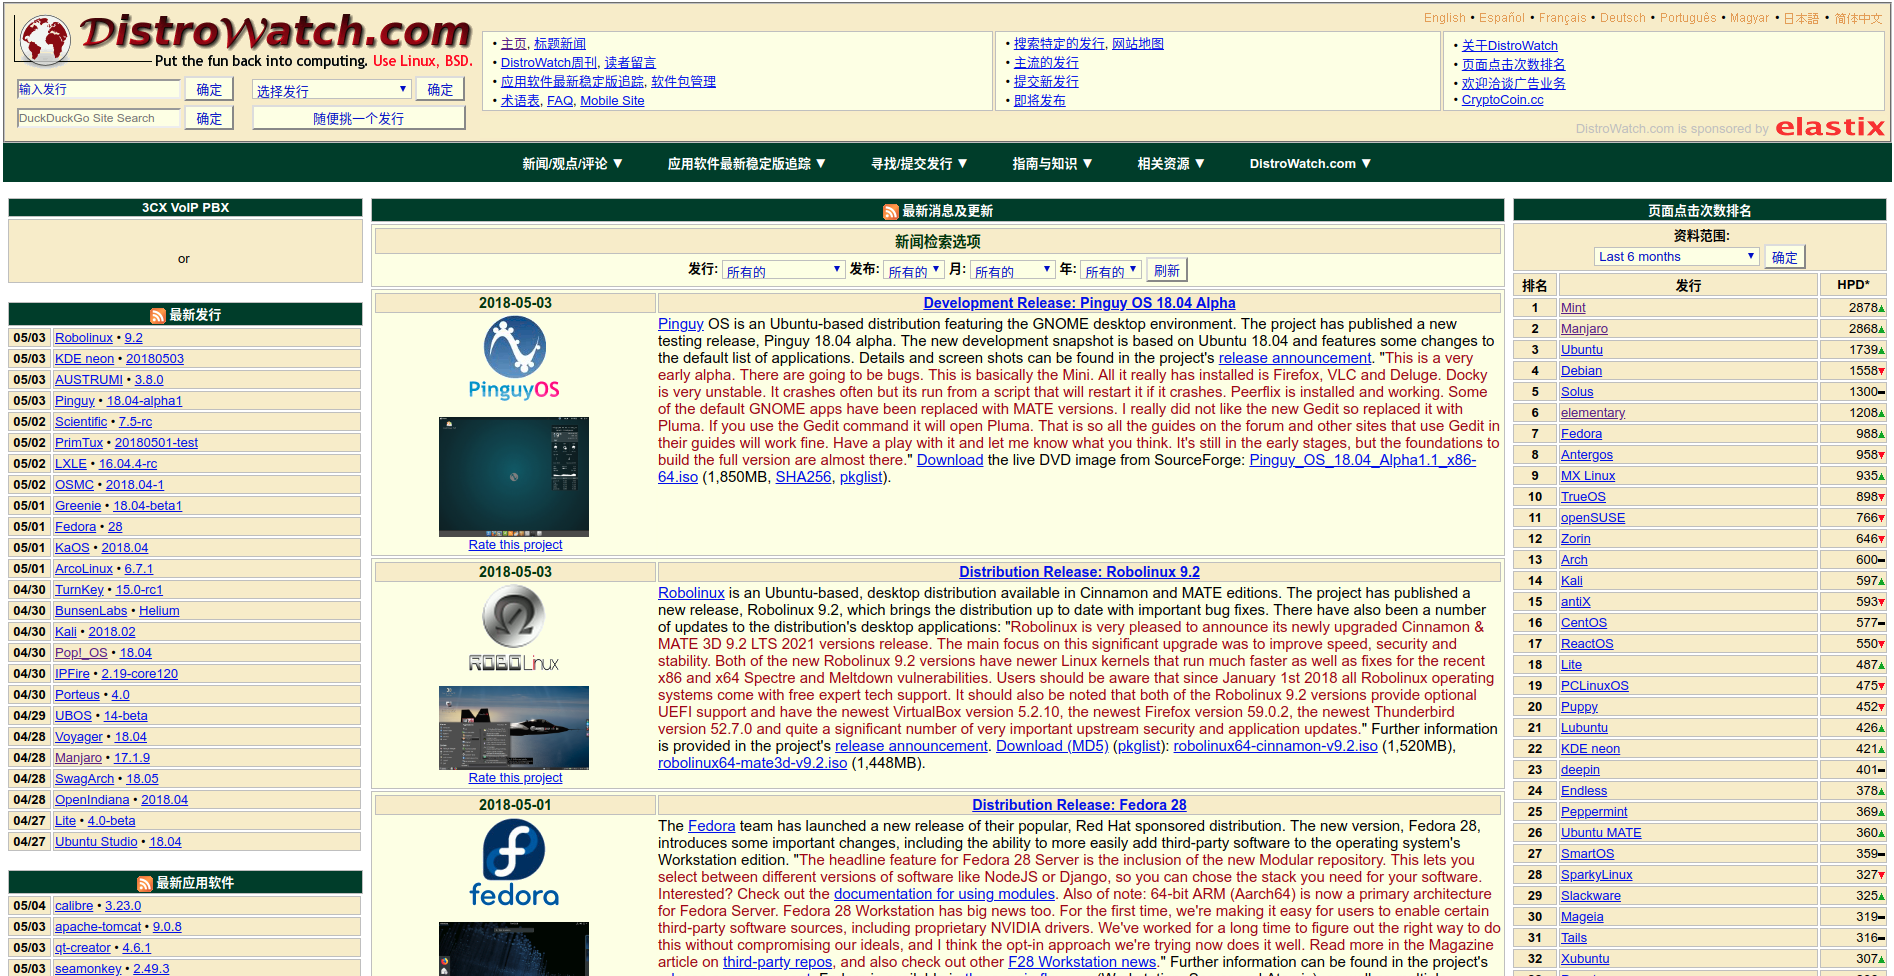
\includegraphics[width=\textwidth]{c1.distrowatch.png}
  \end{figure}
\end{frame}

\subsection{应用领域}
\begin{frame}
  \frametitle{Linux基础 | 简介 | 应用领域}
  \begin{figure}
    \centering
    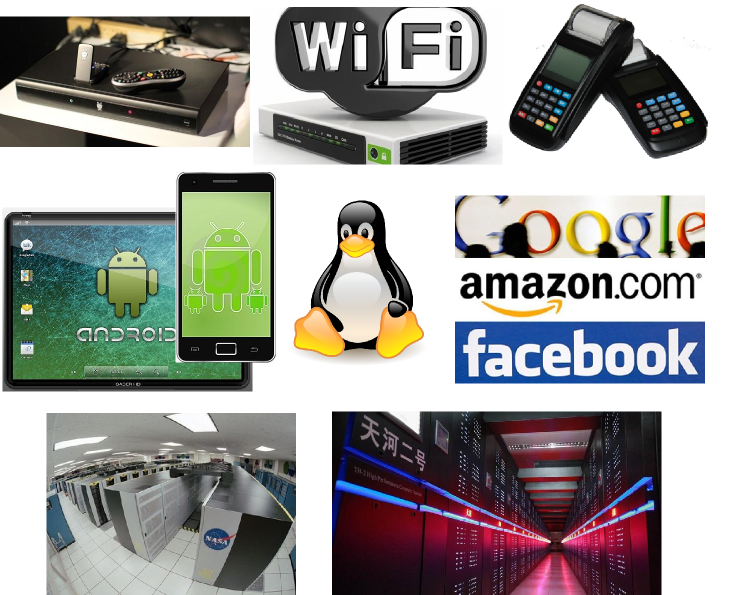
\includegraphics[width=9cm]{c1.linux.area.png}
  \end{figure}
\end{frame}

\begin{frame}
  \frametitle{Linux基础 | 简介 | 应用领域 | 桌面电脑:微乎其微}
  \begin{figure}
    \centering
    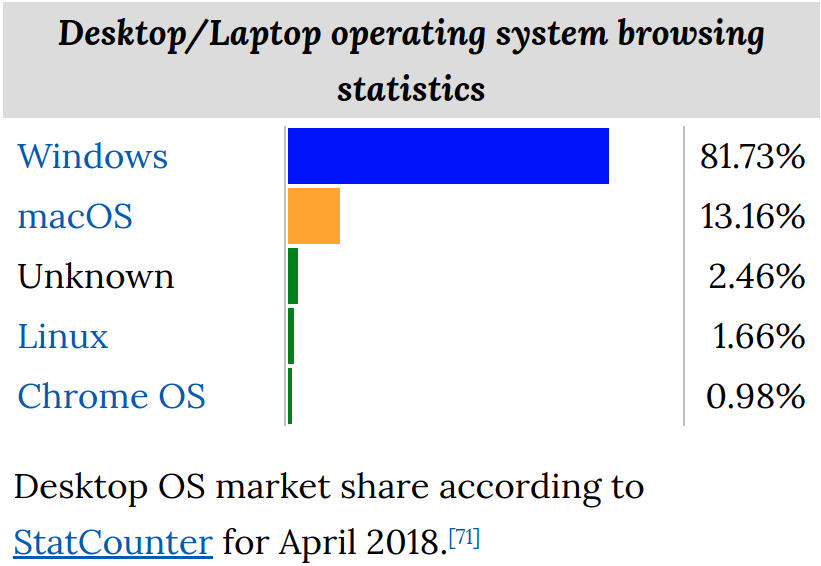
\includegraphics[width=10cm]{c1.linux.area.desktop.2018.png}
  \end{figure}
\end{frame}

\begin{frame}
  \frametitle{Linux基础 | 简介 | 应用领域 | 服务器:三分之二}
  \begin{figure}
    \centering
    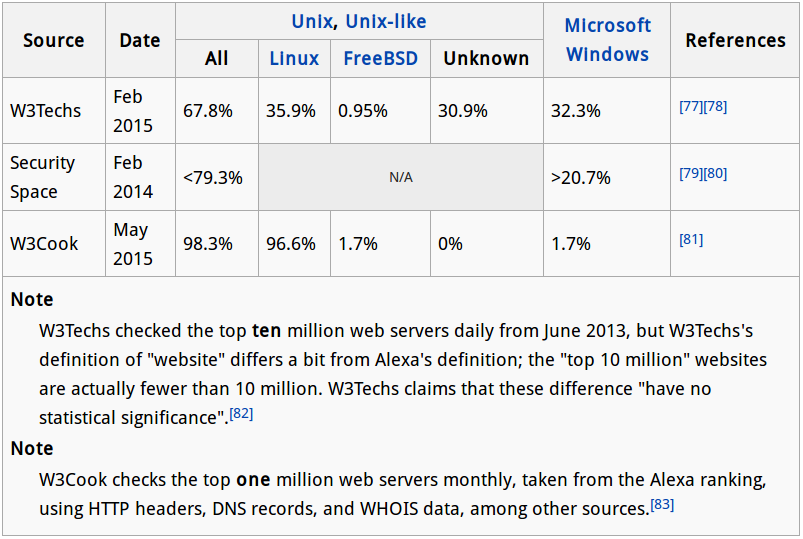
\includegraphics[width=11cm]{c1.linux.area.server.2016.png}
  \end{figure}
\end{frame}

\begin{frame}
  \frametitle{Linux基础 | 简介 | 应用领域 | 智能手机:三分之二}
  \begin{figure}
    \centering
    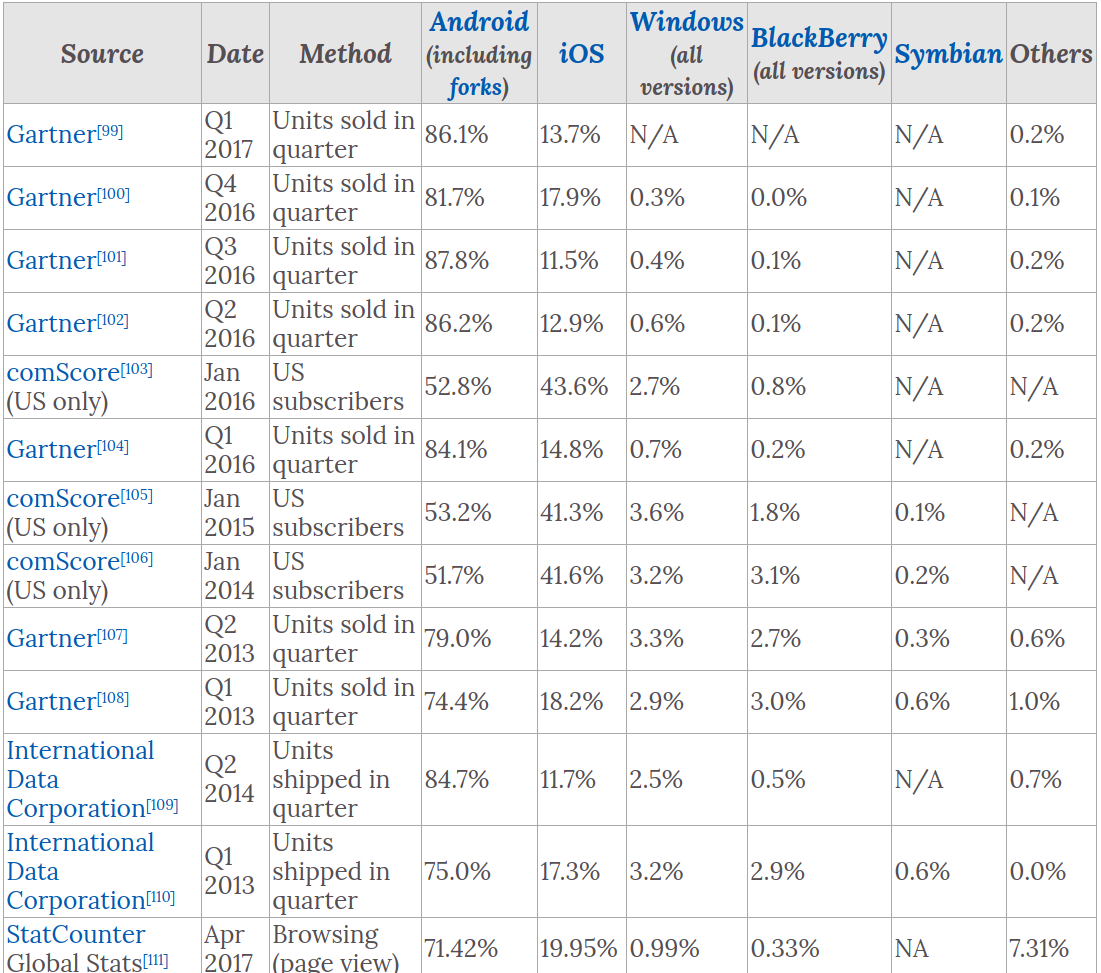
\includegraphics[width=11cm]{c1.linux.area.mobile.2018.png}
  \end{figure}
\end{frame}

\begin{frame}
  \frametitle{Linux基础 | 简介 | 应用领域 | 超级计算机:独领风骚}
  \begin{figure}
    \centering
    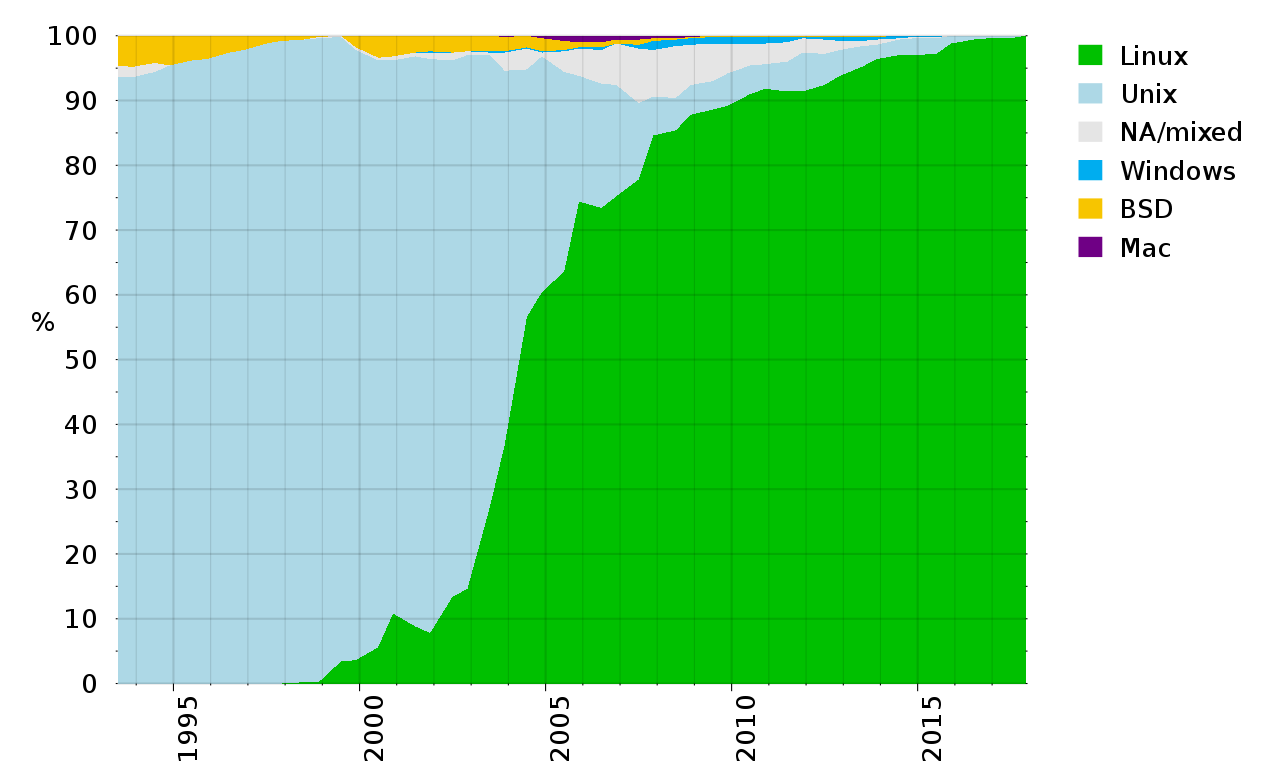
\includegraphics[width=12cm]{c1.linux.area.super.2018.png}
  \end{figure}
\end{frame}

\begin{frame}
  \frametitle{Linux基础 | 简介 | 应用领域 | 分类汇总}
  \begin{figure}
    \centering
    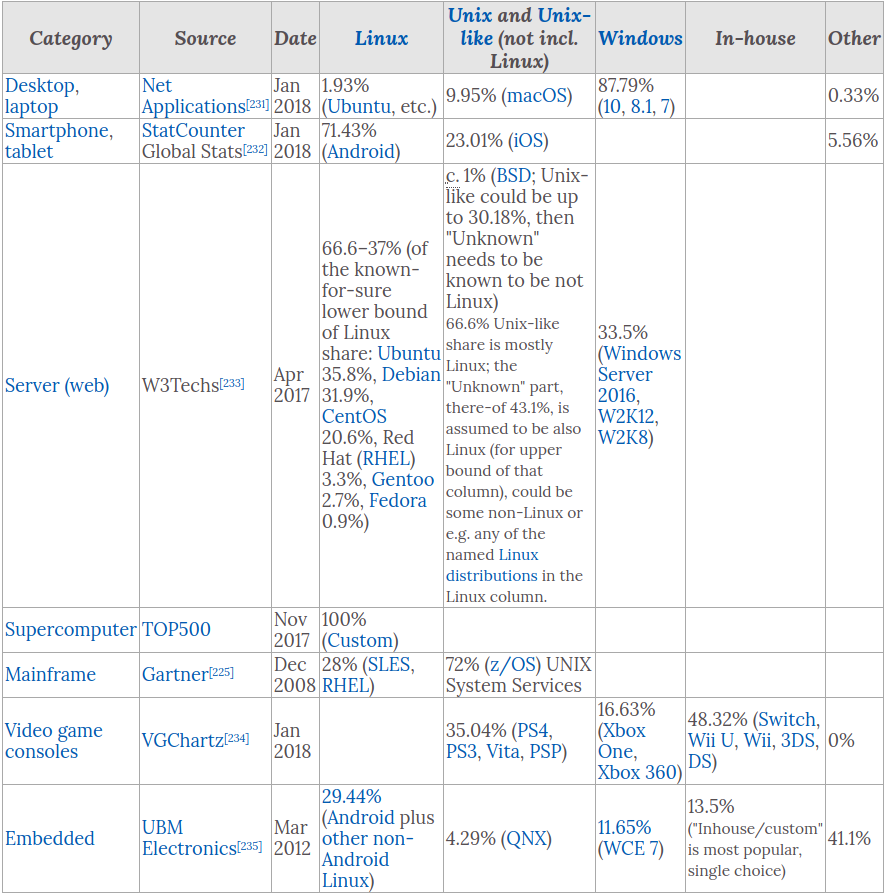
\includegraphics[width=7.5cm]{c1.linux.area.all.2018.png}
  \end{figure}
\end{frame}

\section{操作系统组件}
\begin{frame}
  \frametitle{Linux基础 | 系统组件}
  \begin{block}{Linux操作系统的\alert{构成组件}}
    内核、shell、文件系统和实用程序(应用程序)。
  \end{block}
  \begin{figure}
    \centering
    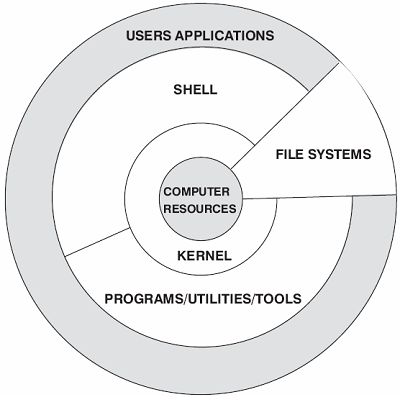
\includegraphics[width=6cm]{c1.system.parts.01.png}
  \end{figure}
\end{frame}

\subsection{内核}
\begin{frame}
  \frametitle{Linux基础 | 系统组件 | 内核}
  \begin{block}{内核}
    内核控制计算机,是操作系统的核心。
  \end{block}
  \pause
  \begin{block}{功能}
  \begin{itemize}
    \item 内存管理(虚拟内存管理,包括页面调度、交换)
    \item 进程管理(进程创建、终止、调度、通信)
    \item 输入/输出(通过设备驱动程序)
    \item 文件管理,网络访问,安全和访问控制
  \end{itemize}
  \end{block}
  \pause
  \begin{block}{版本}
  \begin{itemize}
    \item 版本格式为3.A.B(3.0版本之后,含4.0)
    \item A:内核版本,随新版本的发布而增加
    \item B:安全补丁,bug修复、安全更新、新特性和驱动的次数
  \end{itemize}
  \end{block}
\end{frame}

\subsection{shell}
\begin{frame}
  \frametitle{Linux基础 | 系统组件 | shell}
  \begin{block}{shell}
    shell是一个命令行解释器,它使得用户能够与操作系统进行交互。
  \end{block}
  \pause
  \begin{block}{\alert{种类}}
  %\begin{itemize}[<+-|alert@+>]
  \begin{itemize}[<+->]
    \item sh(Bourne shell):Unix的第一个shell
    \item bash(Bourne-Again shell):Bourne shell的后继相容版本与开放源代码版本
    \item dash(Debian Almquist shell):快而轻巧,兼容于POSIX标准
    \item zsh(Z shell):一种Bourne shell的扩展,带有数量庞大的改进
    \item csh(C shell):语法类似于C语言;tcsh:csh的增强版本
    \item ksh(Korn shell):完全向上兼容Bourne shell并包含了C shell的很多特性
  \end{itemize}
  \end{block}
\end{frame}

\subsection{其他组件}
\begin{frame}
  \frametitle{Linux基础 | 系统组件 | 其他}
  \begin{block}{文件系统}
    使得用户能够以统一的方式查看、组织以及保护存储设备上的文件和目录并与其进行交互。
  \end{block}
  \pause
  \begin{block}{实用程序}
    使得用户能够在系统上进行工作,包括Web浏览器、文字处理程序、e-mail程序等应用程序。
  \end{block}
\end{frame}

\section{Linux的学习}
\subsection{安装Linux}
\begin{frame}
  \frametitle{Linux基础 | 学习 | 安装}
  %\begin{enumerate}[<+-|alert@+>]
  \begin{enumerate}[<+->]
    \item Live CD:一个可引导的CD-ROM,包含运行一个完整操作系统所需的所有内容:内核、实用工具等
    \item Live USB:类似于Live CD,但可以更改设置、保存文件、安装软件
    \item \alert{MultiBootUSB}:MultiBootUSB is a cross platform software written in python which allows you to install multiple live linux on a USB disk non destructively and option to uninstall distros.
    \item 硬盘安装\textcolor{red}{(谨慎选择,尤其是品牌机笔记本)}
      \begin{itemize}
        \item \textcolor{gray}{Wubi(基于Windows的安装程序,Windows-based Ubuntu Installer),DeepWin:无需对硬盘进行格式化或重新分区}
        \item 虚拟机:在实体计算机上,使用宿主机的硬件资源,通过软件模拟出一台或者多台虚拟计算机,拥有真实计算机的绝大多数功能
        \item 多重引导系统:在计算机上安装不止一个操作系统,但一次只能运行一个操作系统,切换时需要重新启动计算机
        \item 单系统:在计算机上只安装一个操作系统
      \end{itemize}
  \end{enumerate}
\end{frame}

\begin{frame}
  \frametitle{Linux基础 | 学习 | 安装 | MultiBootUSB}
  \begin{figure}
    \centering
    \includegraphics[width=7.8cm]{c1.multibootusb.png}
  \end{figure}
\end{frame}

\begin{frame}
  \frametitle{Linux基础 | 学习 | 安装 | 虚拟机 | VirtualBox}
  \begin{figure}
    \centering
    \includegraphics[width=10cm]{c1.virtualbox.01.png}
  \end{figure}
\end{frame}

\begin{frame}
  \frametitle{Linux基础 | 学习 | 安装 | 虚拟机 | VMware Player}
  \begin{figure}
    \centering
    \includegraphics[width=9cm]{c1.vmware.01.jpg}
  \end{figure}
\end{frame}

\begin{frame}
  \frametitle{Linux基础 | 学习 | 安装 | \textcolor{gray}{容器 | Docker}}
  \begin{block}{Docker简介}
    Docker是一个开放源代码软件专案,在软件容器下自动布署应用程序,借此\textbf{在Linux操作系统上},提供了一个额外的软件抽象层,以及操作系统层虚拟化的自动管理机制。Docker利用Linux内核中的资源分离机制,例如cgroups、以及Linux内核名称空间,来建立独立的软件容器(containers)。这可以在单一Linux实体下运作,避免启动一个虚拟机器造成的额外负担。
  \end{block}
  \pause
  \begin{block}{安装使用}
    \begin{enumerate}
      \item 安装Docker:sudo apt-get install docker.io,sudo yum install docker
      \item 获取镜像:sudo docker pull ubuntu:18.04(centos:centos7,……)
      \item 启动容器:sudo docker run -t -i ubuntu:18.04(centos:centos7) /bin/bash
    \end{enumerate}
  \end{block}
\end{frame}

\subsection{学习Linux}
\begin{frame}[fragile]
  \frametitle{Linux基础 | 学习 | GUI vs. CLI}
  \begin{verbatim}
Graphical user interfaces make easy tasks easier,
while command line interfaces make difficult tasks
possible.
  \end{verbatim}
  \vspace{-0.8cm}
  \begin{figure}
    \centering
    %\includegraphics[width=8cm]{c1.gui.jpg}\\
    %\includegraphics[width=8cm]{c1.cli.png}
    \includegraphics[width=11cm]{c1.gui.cli.png}
  \end{figure}
\end{frame}

\begin{frame}
  \frametitle{Linux基础 | 学习 | GUI vs. CLI}
  \begin{block}{\alert{用户界面}}
    %\begin{itemize}[<+-|alert@+>]
    \begin{itemize}[<+->]
      \item 图形用户界面(Graphical User Interface,简称GUI)是指采用图形方式显示的计算机操作用户界面。
      \item 命令行界面(Command Line Interface,简写CLI)是在图形用户界面得到普及之前使用最为广泛的用户界面,它通常不支持鼠标,用户通过键盘输入指令,计算机接收到指令后,予以执行。
    \end{itemize}
  \end{block}
  \pause
  \begin{block}{界面比较}
    \begin{itemize}
      \item GUI对于用户来说在视觉上更易于接受,操作简单而且直观;在不同系统间、不同发行版间差异大,不能完成所有的操作任务。
      \item CLI占用资源少,启动迅速,操作更加高效,可以完成所有的工作,不同系统间、不同发行版间具有高度的相似性。
    \end{itemize}
  \end{block}
  \pause
\end{frame}

\begin{frame}
  \frametitle{Linux基础 | 学习 | 策略与步骤}
  \begin{block}{策略}
    学习 + 摸索 + 实践 + 总结
  \end{block}
  \pause
  \begin{block}{步骤}
    %\begin{enumerate}[<+-|alert@+>]
    \begin{enumerate}[<+->]
      \item 计算机概论
      \item Linux的安装/远程连接与命令
      \item Linux操作系统的基本技能:用户/用户组,权限
      \item vi文本编辑器
      \item shell与shell脚本:正则表达式,管道,重定向
      \item 软件与系统管理:dpkg/RPM/tarball
    \end{enumerate}
  \end{block}
\end{frame}

\begin{frame}
  \frametitle{Linux基础 | 学习 | 方法}
  \begin{block}{方法}
    %\begin{itemize}[<+-|alert@+>]
    \begin{itemize}[<+->]
      \item 忘记Windows的思维方式
      \item GUI是表象,CLI是本质
      \item 注意系统的提示信息,自行解决“疑难杂症”
      \begin{itemize}
        \item Command not found
        \item No such file or directory
        \item Permission denied
      \end{itemize}
      \item 在自己的电脑/网络上查询How-To或FAQ
      \begin{itemize}
        \item RTFM:Read The Fine/Friendly/Foolish/F**king Manual
        \item STFW:Search The F**king Web
        \item UTFG:Use The F**king Google
      \end{itemize}
      \item 查询后,注意网络礼节,在论坛/讨论群里大胆提问、发言
      \begin{itemize}
        % \item \href{http://www.wapm.cn/smart-questions/smart-questions-zh.html}{提问的智慧(How To Ask Questions The Smart Way)}
        % \item \href{http://code.google.com/p/cpyug/wiki/ZenForAsk}{回答的智慧}
        \item \href{https://github.com/ryanhanwu/How-To-Ask-Questions-The-Smart-Way/blob/master/README-zh_CN.md}{提问的智慧(How To Ask Questions The Smart Way)}
        \item \href{http://dbanotes.net/tech-memo/how_to_answer_questions_the_smart_way.html}{回答的智慧}
        \item \href{https://blog.m157q.tw/posts/2017/12/21/how-to-answer-questions-in-a-helpful-way-zh-tw/}{回答的智慧}
      \end{itemize}
    \end{itemize}
  \end{block}
\end{frame}

\begin{frame}
  \frametitle{Linux基础 | 学习 | 方法 | 提问}
  \begin{figure}
    \centering
    \includegraphics[width=0.8\textwidth]{c1.asking.png}
  \end{figure}
\end{frame}

\begin{frame}
  \frametitle{Linux基础 | 学习 | 方法 | 提问}
    \begin{block}{提问前}
      \begin{itemize}
        \item 尝试搜索答案——官网/手册/FAQ/Google/论坛
        \item 尝试自己检查或试验以找到答案
        \item 尝试阅读源代码以找到答案
      \end{itemize}
    \end{block}
    \pause
    \begin{block}{提问}
      \begin{itemize}
        \item 清楚明确得表达你的问题以及需求,描述目标而不是过程
        \item 按发生时间先后列出问题症状,描述问题症状而非你的猜测
        \item 提供最精简的Bug展示测试用例(bug-demonstrating test case)
        \item 即使你很急也不要在标题写“紧急”,问题解决后加个简短的补充说明
      \end{itemize}
    \end{block}
\end{frame}

\begin{frame}
  \frametitle{Linux基础 | 学习 | 方法 | 提问 | 实例}
  \begin{block}{蠢问题}
    \begin{itemize}
      \item 救命啊!我的笔记本电脑不能正常显示了!
      \item 我可以在哪儿找到关于Foonly Flurbamatic的资料?
      \item 我的主机板有问题了,谁来帮我?
      % \item 我从foo项目找来的源码没法编译。它怎么这么烂?
    \end{itemize}
  \end{block}
  \pause
  \vspace{-0.5em}
  \begin{block}{聪明问题}
    \begin{itemize}
      \item X.org 6.8.1的鼠标光标,在某牌显卡MV1005芯片组环境下——会变形。
      \item 我用Google搜索过``Foonly Flurbamatic 2600",但是没找到有用的结果。谁知道上哪儿去找对这种设备编程的资料
      \item 我在S2464主机板上试过了X、Y和Z,但没什么作用,我又试了A、B和C。请注意当我尝试C时的奇怪现象。显然florbish正在grommicking,但结果出人意料。通常在Athlon MP主机板上引起grommicking的原因是什么?有谁知道接下来我该做些什么测试才能找出问题?
      % \item foo项目代码在Nulix 6.2版下无法编译通过。我读过了FAQ,但里面没有提到跟Nulix有关的问题。这是我编译过程的记录,我有什么做的不对的地方吗?
    \end{itemize}
  \end{block}
\end{frame}

\begin{frame}
  \frametitle{Linux基础 | 学习 | 方法 | 提问 | 实例}
  \begin{figure}
    \centering
    \includegraphics[width=0.35\textwidth]{c1.asking.weixin.01.png}
    \includegraphics[width=0.25\textwidth]{c1.asking.weixin.02.png}
    \includegraphics[width=0.35\textwidth]{c1.asking.weixin.03.png}
  \end{figure}
\end{frame}

\section{Linux起步}
\subsection{登录Linux}
\begin{frame}
  \frametitle{Linux基础 | 起步 | 登录 | GUI登录}
  \begin{figure}
    \centering
    \includegraphics[width=9cm]{c1.login.gui.png}
  \end{figure}
\end{frame}

\begin{frame}
  \frametitle{Linux基础 | 起步 | 登录 | 命令行登录}
  \begin{figure}
    \centering
    \includegraphics[width=9.5cm]{c1.login.cli.png}
    \vspace{0.1cm}
    \includegraphics[width=9.5cm]{c1.login.cli.error.jpg}
  \end{figure}
\end{frame}

\begin{frame}
  \frametitle{Linux基础 | 起步 | 登录 | 命令行登录 | 安全特性}
  %\begin{itemize}[<+-|alert@+>]
  \begin{itemize}[<+->]
    \item 登录时不提示可用的用户名有哪些
    \item 输入的密码不显示(长度、字符)
    \item Login incorrect:不提示用户名无效还是密码错误
    \item 显示用户上一次登录的时间
  \end{itemize}
\end{frame}

\begin{frame}[fragile]
  \frametitle{Linux基础 | 起步 | 登录 | 远程登录}
  \begin{table}
    \centering
    \rowcolors[]{1}{blue!20}{blue!10}
    \begin{tabular}{clll}
      \hline
      \rowcolor{blue!50}命令 & 功能 & 加密 & 示例\\
      \hline
      \alert{ssh} & 运行命令 & 加密 & ssh \textcolor{gray}{USERNAME@}HOSTNAME\\
      telnet & 运行命令 & 不加密 & telnet HOSTNAME(名称或IP)\\
      sftp & 传输文件 & 加密 & ---\\
      ftp & 传输文件 & 不加密 & ---\\
      \hline
    \end{tabular}
  \end{table}
  \pause
  \begin{block}{ssh实例}
    \begin{itemize}
      \item \verb|ssh 000.000.000.000|
      \item \verb|ssh zhangsan@000.000.000.000|
      \item \verb|passwd|
      \item \verb|passwd zhangsan|
    \end{itemize}
  \end{block}
\end{frame}

\begin{frame}
  \frametitle{Linux基础 | 起步 | 登录 | 远程登录 | Windows | SSH}
  \begin{block}{PuTTY}
    PuTTY是一款集成虚拟终端、系统控制台和网络文件传输为一体的免费且开源的程序。它支持多种网络协议,包括SCP,SSH,Telnet,rlogin和原始的套接字连接。\\
    % PuTTY is an SSH and telnet client, developed originally by Simon Tatham for the Windows platform. PuTTY is open source software that is available with source code and is developed and supported by a group of volunteers.
  \end{block}
  \begin{figure}
    \centering
    \includegraphics[width=0.45\textwidth]{c1.putty.01.png}
    \includegraphics[width=0.45\textwidth]{c1.putty.02.jpg}
  \end{figure}
\end{frame}

\begin{frame}
  \frametitle{Linux基础 | 起步 | 登录 | 远程登录 | Windows | SSH}
  \begin{block}{MobaXterm}
    Enhanced terminal for Windows with X11 server, tabbed SSH client, network tools and much more.
  \end{block}
  \begin{figure}
    \centering
    \includegraphics[width=0.75\textwidth]{c1.mobaxterm.01.png}
  \end{figure}
\end{frame}

\begin{frame}
  \frametitle{Linux基础 | 起步 | 登录 | 远程登录 | Windows | FTP}
  \begin{block}{FileZilla}
    FileZilla是一种快速、可信赖的FTP客户端以及服务器端开放源代码程序,具有多种特色、直觉的接口。
  \end{block}
  \begin{figure}
    \centering
    \includegraphics[width=0.85\textwidth]{c1.filezilla.01.png}
  \end{figure}
\end{frame}

\begin{frame}
  \frametitle{Linux基础 | 起步 | 登录 | 远程登录 | Windows}
  \begin{block}{资源网站}
    \begin{itemize}
      \item \href{https://www.wikiwand.com/zh-cn/SSH\%E5\%AE\%A2\%E6\%88\%B7\%E7\%AB\%AF\%E6\%AF\%94\%E8\%BE\%83}{SSH客户端比较}
      \item \href{https://www.wikiwand.com/zh-cn/FTP\%E5\%AE\%A2\%E6\%88\%B7\%E7\%AB\%AF\%E6\%AF\%94\%E8\%BE\%83}{FTP客户端比较}
      \item \href{https://www.putty.org/}{PuTTY}
      \item \href{https://mobaxterm.mobatek.net/}{MobaXterm}
      \item \href{https://filezilla-project.org/}{FileZilla}
      \item \href{https://freefilesync.org/}{FreeFileSync: Synchronize Files and Folders}
    \end{itemize}
  \end{block}
  \pause
  \begin{block}{常用端口}
    \begin{itemize}
      \item 21:FTP
      \item 22:SSH
      \item 其他:23——Telnet;80——HTTP;443——HTTPS
    \end{itemize}
  \end{block}
\end{frame}

\begin{frame}
  \frametitle{Linux基础 | 起步 | 上机实习环境}
  \begin{block}{简单}
    直接使用机房中的台式机(\alert{警告:每次重启自动还原})
  \end{block}
  \pause
  \begin{block}{推荐}
    \begin{itemize}
      \item 使用机房台式机中的预装Windows系统\\ \quad U盘 + 便携版Windows相关软件(PuTTY/MobaXterm+FileZilla)
      \item 使用机房台式机进入U盘Linux系统\\ \quad U盘(>=8G)+ MultiBootUSB(LinuxMint/Ubuntu/Fedora/...)
    \end{itemize}
  \end{block}
  \pause
  \begin{block}{其他}
    自带笔记本(预装Linux/预装Windows相关软件)
  \end{block}
\end{frame}

\subsection{退出Linux}
\begin{frame}
  \frametitle{Linux基础 | 起步 | 退出与关闭}
  \begin{table}
    \centering
    \rowcolors[]{1}{blue!20}{blue!10}
    \begin{tabular}{cl}
      \hline
      \rowcolor{blue!50}命令 & 功能\\
      \hline
      exit(Ctrl + D) & 结束shell会话\\
      logout(Ctrl + D) & 退出系统\\
      \hline
      shutdown & 关闭系统\\
      \alert{shutdown -h} & 关闭计算机,halt + poweroff\\
      shutdown -r & 关闭和重启系统,reboot\\
      \alert{reboot} & 重新启动系统\\
      poweroff & 通过切断电源来关闭系统\\
      halt & 立即关闭系统\\
      init 0 & 切断系统电源(在关机前同步数据并整理系统)\\
      init 6 & 将系统完全关闭后重新启动系统\\
      \hline
    \end{tabular}
  \end{table}
\end{frame}

\subsection{联机帮助页}
\begin{frame}
  \frametitle{Linux基础 | 起步 | 手册}
  \begin{block}{联机帮助页(man pages)}
    联机帮助页,帮助文件,手册,man pages,manual pages
  \end{block}
  \pause
  \begin{table}
    \centering
    \rowcolors[]{1}{blue!20}{blue!10}
    \begin{tabular}{cl}
      \hline
      \rowcolor{blue!50}命令 & 功能\\
      \hline
      \alert{man COMMAND} & 查看COMMAND的联机帮助页\\
      man man & 查看man的联机帮助页\\
      \hline
      \alert{man -k KEYWORD} & 根据关键字搜索联机帮助页\\
      man -k permission & 查找权限的相关命令\\
      man -k manual & 查找手册的相关命令\\
      man -k shell & 查找shell的相关命令\\
      \hline
    \end{tabular}
  \end{table}
\end{frame}

\begin{frame}
  \frametitle{Linux基础 | 起步 | 手册}
  \begin{figure}
    \centering
    \includegraphics[width=11cm]{c1.man.png}
  \end{figure}
\end{frame}

\begin{frame}
  \frametitle{Linux基础 | 起步 | 手册}
  \begin{figure}
    \centering
    \includegraphics[width=10cm]{c1.man.page.02.png}
  \end{figure}
\end{frame}

\begin{frame}
  \frametitle{Linux基础 | 起步 | 手册 | 解释}
  \begin{table}
    \centering
    \rowcolors[]{1}{blue!20}{blue!10}
    \begin{tabular}{cl}
      \hline
      \rowcolor{blue!50}部分 & 解释\\
      \hline
      NAME & 命令的名称\\
      SYNOPSIS & 命令的使用格式与常用参数\\
      DESCRIPTION & 命令的作用描述\\
      OPTIONS & 命令所有的参数或选项\\
      SEE ALSO & 与该命令相关或功能相近的其他命令\\
      BUGS & 存在的已知问题或缺陷\\
      EXAMPLES/TIPS & 命令的用法示例\\
      AUTHORS & 联机帮助页/命令的作者\\
      \hline
    \end{tabular}
  \end{table}
\end{frame}

\begin{frame}
  \frametitle{Linux基础 | 起步 | 手册 | 解释}
  \begin{figure}
    \centering
    \includegraphics[width=11.5cm]{c1.man.page.01.png}
  \end{figure}
\end{frame}

\section{回顾与总结}
\subsection{总结}
\begin{frame}
  \frametitle{Linux基础 | 总结}
  \begin{block}{知识点}
    \begin{itemize}
      \item Linux的历史与现状
      \item Linux的含义
      \item Linux发行版
      \item 操作系统组件
      \item Linux的登录与退出
      \item Linux的联机帮助页
    \end{itemize}
  \end{block}
  \begin{block}{技能}
    \begin{itemize}
      \item \textcolor{gray}{VirtualBox虚拟机的使用}
      \item \textcolor{gray}{Linux系统的安装}
      \item 远程连接Linux服务器
      \item Linux系统的学习
    \end{itemize}
  \end{block}
\end{frame}

\subsection{思考题}
\begin{frame}
  \frametitle{Linux基础 | 思考题}
  \begin{enumerate}
    \item Unix和Linux分别是由谁开发的?
    \item Linux发行版主要分成哪两大系统?
    \item 列举几个常见的Linux发行版。
    \item Linux操作系统主要包括哪些组件?
    \item 列举几种常见的shell。
    \item 登录、退出、关闭Linux的常用命令。
    \item 如何查看命令的联机帮助页?
    \item 如何根据关键字查找相关命令?
  \end{enumerate}
\end{frame}

\begin{frame}
  \frametitle{下节预告}
  \begin{block}{普遍问题}
    对于一个机构或组织,如何分配权限?如何共享及保密信息?
  \end{block}
  \pause
  \begin{block}{具体问题}
    假设一家公司,有大约100个员工,包括管理层、人力资源部门、研发部门、普通员工等,如何规划才能保证管理层、人力资源部门可以查阅并处理工资、人事调动等敏感信息,同时还能防止普通员工获取到这些信息?与之类似,如何保证研发部门能获得最新的公司的技术研发机密,而对其他人进行保密?
  \end{block}
  \pause
  \begin{block}{解答提示}
    机密安全等级(Clearance Level)(《神盾局特工》),部门分配,组别划分,……
  \end{block}
\end{frame}




\section*{Acknowledgements}
\begin{frame}
  \frametitle{Powered by}
  \begin{center}
    \includegraphics[width=9cm]{power.png}
  \end{center}
\end{frame}

\end{document}

